\chapter{Simulation and Results}
\label{chap:5_Simulation_And_Results}
    
        %V1.0:
        % In this chapter, we present scenarios for validation and evaluation and experimental results. The scenarios cover different encounters between vessels for collision avoidance evaluation and for identification of our system's response and limitations we expose it to different wind speeds. Beyond that, we present the execution with and without \ac{ATC} for scientific control validation of the path planning algorithm. As done by several authors, \eg{} Larson \etal{} ~\cite{Larson2006Autonomous}, Naeem \etal{} ~\cite{Naeem2012COLREGS}, Campbell \etal{} ~\cite{Campbell2013Automatic}, Naus ~\cite{Naus2013Idea}, \etc{}, we evaluated 4 main encounter scenarios between two vessels: head-on, crossing from right, crossing from left and overtaking. Based on \cite{} we made a quantitative evaluation of our planning system measuring computational cost and minimum distance between vessels.
        
        %V2.0:
        % In this chapter, we present scenarios for validation (qualitative analysis) and evaluation (quantitative analysis) and experimental results. The scenarios cover different encounters between vessels for collision avoidance success evaluation and exposition to different environmental behaviors for identification of response capability and limitations of our system. Beyond that, we present the execution with and without \ac{ATC} for scientific control validation of our path planning algorithm.
        
        %V3.0:
        % In this chapter, we present the scenarios for validation (qualitative analysis) and evaluation (quantitative analysis) and experimental results. The scenarios cover different encounters between vessels for collision avoidance success evaluation and exposition to different environmental behaviors for identification of response capability and limitations of our system. Beyond that, we present the execution of our path planning algorithm with and without \ac{ATC}.
        
        %V4.0:
        In this chapter, we present the scenarios for validation (qualitative analysis) and evaluation (quantitative analysis) of our approach, as well as the experimental results. The simulations cover different encounters scenarios between vessels for evaluation of collision avoidance success and exposition to different environmental behaviors for identification of limitations of our system.

    \section{Simulations Characterization}
    
    We run our simulations on \usvsim ~\cite{Paravisi2018Toward} simulator using the platform described in Table \ref{tab:simulation_platform_description}. 
    %Grammarlly: 100/100
    We developed 12 scenarios for evaluation the system focusing on being comparable with simulations presented in reference studies, \ie{} Agrawal \etal{} ~\cite{Agrawal2015COLREGS} and Huang \etal{} ~\cite{Huang2019Generalized}. Both studies were chosen for their quality ( \ie{} h-index) and similarity with our work. Agrawal \etal{} was chosen for being our problem-solving inspiration. Unfortunately, they do not present too much information about their system evaluation, so we based our tests and system evaluation on Huang \etal{} as they explicitly present their simulation scenarios characterization, results, and simulate a \ac{USV} similar in dimensions to ours.
    
    \taburowcolors[1] 1{tableLineOne .. tableLineTwo}
    \tabulinesep = ^3mm_2mm
    \everyrow{\tabucline[.4mm  white]{}}

    \begin{table}
        \caption{Simulation Platform Description}
        \centering
            \begin{tabu} to \textwidth { >{\bfseries}X[c, 0] X[c, 3]}
            Computer & Desktop Dell XPS 8700 \\
            Processor & Intel® Core™ i7-4770 CPU @ 3.40GHz × 8 \\
            Memory & \begin{tabular}[c]{@{}l@{}}Teikon PC3-12800u DDR3 1600 MHz 2GB x 2\\ Teikon PC3-12800u DDR3 1600 MHz 4GB x 2\end{tabular} \\
            Operating System & Ubuntu 16.04.6 LTS \\
            ROS Version & ROS Kinetic
            \end{tabu}  
        \label{tab:simulation_platform_description}
    \end{table}
    
        % Grammarlly: 100/100
    In our simulations, we use a differential boat - shown in Figure \ref{fig:diffboat} - with two thrusters, which enables it to rotate over its axis. This boat is modeled according to specifications of the Lutra Prop boat, acquired from Platypus ~\cite{PlatypusLLC}. The differential boat is 106 centimeters long\footnote{Our comparing reference, \ie{} Huang \etal{} \cite{Huang2019Generalized} evaluate a 120 centimeters long vessel}, 48 centimeters wide and 15 centimeters tall, being able to achieve a maximum speed of 1.14 m/s. In its bow, we simulate a parameterized laser for environment scanning, allowing us to set different angles and detection distance ranges.
    
    \begin{figure}[H]
        \centering
        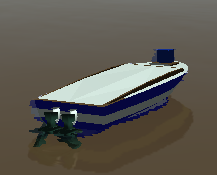
\includegraphics[scale=0.75]{figs/diffboat.png}
        \caption{Simulated version of Lutra Prop boat}
        \label{fig:diffboat}
    \end{figure}
%AMA acho q apresentacao do barco deva vir antes da apresentacao dos 4 cenarios. vc deve mencionar outras caracteristicas, como peso, sensores, a caracteristicas do laser.  

    
    
     We assembled the scenarios in a simulated version of the Dilúvio stream (see Figures \ref{fig:simulation_diluvio_googleLocation_roundedArea}, \ref{fig:simulation_diluvio_googleLocation2_1_roundedArea} and \ref{fig:simulation_diluvio_googleLocation2_2_roundedArea}), and as done by several authors, \eg{} Larson \etal{} ~\cite{Larson2006Autonomous}, Naeem \etal{} ~\cite{Naeem2012COLREGS}, Campbell \etal{} ~\cite{Campbell2013Automatic}, Naus ~\cite{Naus2013Idea}, \etc{}, we evaluated 4 main encounter scenarios between two vessels, head-on, crossing from right, crossing from Left, and overtaking. Figures \ref{fig:simulation_uwsim_headon_starting_pos}, \ref{fig:simulation_uwsim_crossingright_starting_pos}, \ref{fig:simulation_uwsim_crossingleft_starting_pos} and \ref{fig:simulation_uwsim_overtake_starting_pos} show the starting configuration of the evaluated scenarios, the respective configuration of each scenario is presented in Tables \ref{tab:simulation_scenarios_configuration_own_vessel} and \ref{tab:simulation_scenarios_configuration_encountering_vessel}.
    
    \begin{figure}[H]
        \centering
        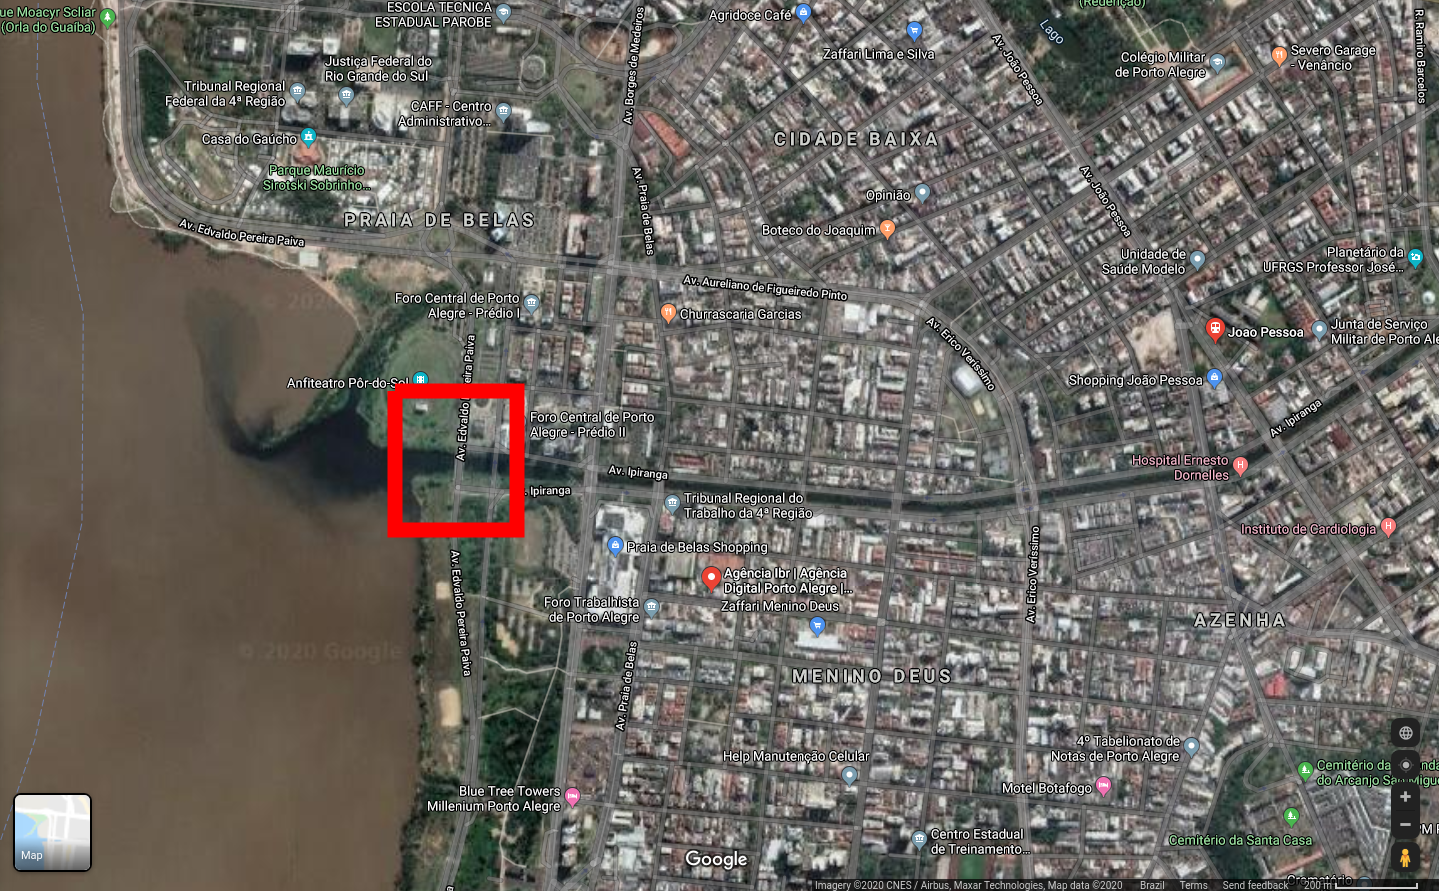
\includegraphics[scale=0.3]{figs/simulation_diluvio_googleLocation_roundedArea.png}
        \caption{Real-world location of the area we choose for evaluation of our system. This is a potential place for real-world trials of our system, once it has and is near our laboratory, so we evaluate the behavior of our system on it. Google maps location (-30.047258°, -51.232660°), Av. Edvaldo Pereira Paiva, 1970 - Praia de Belas - Porto Alegre - RS - Brazil}
        \label{fig:simulation_diluvio_googleLocation_roundedArea}
    \end{figure}
    \todo{cite some characteristics of the region}
    
    \begin{figure}[H]
    \centering
        \begin{subfigure}[b]{0.5\textwidth}
            \centering
            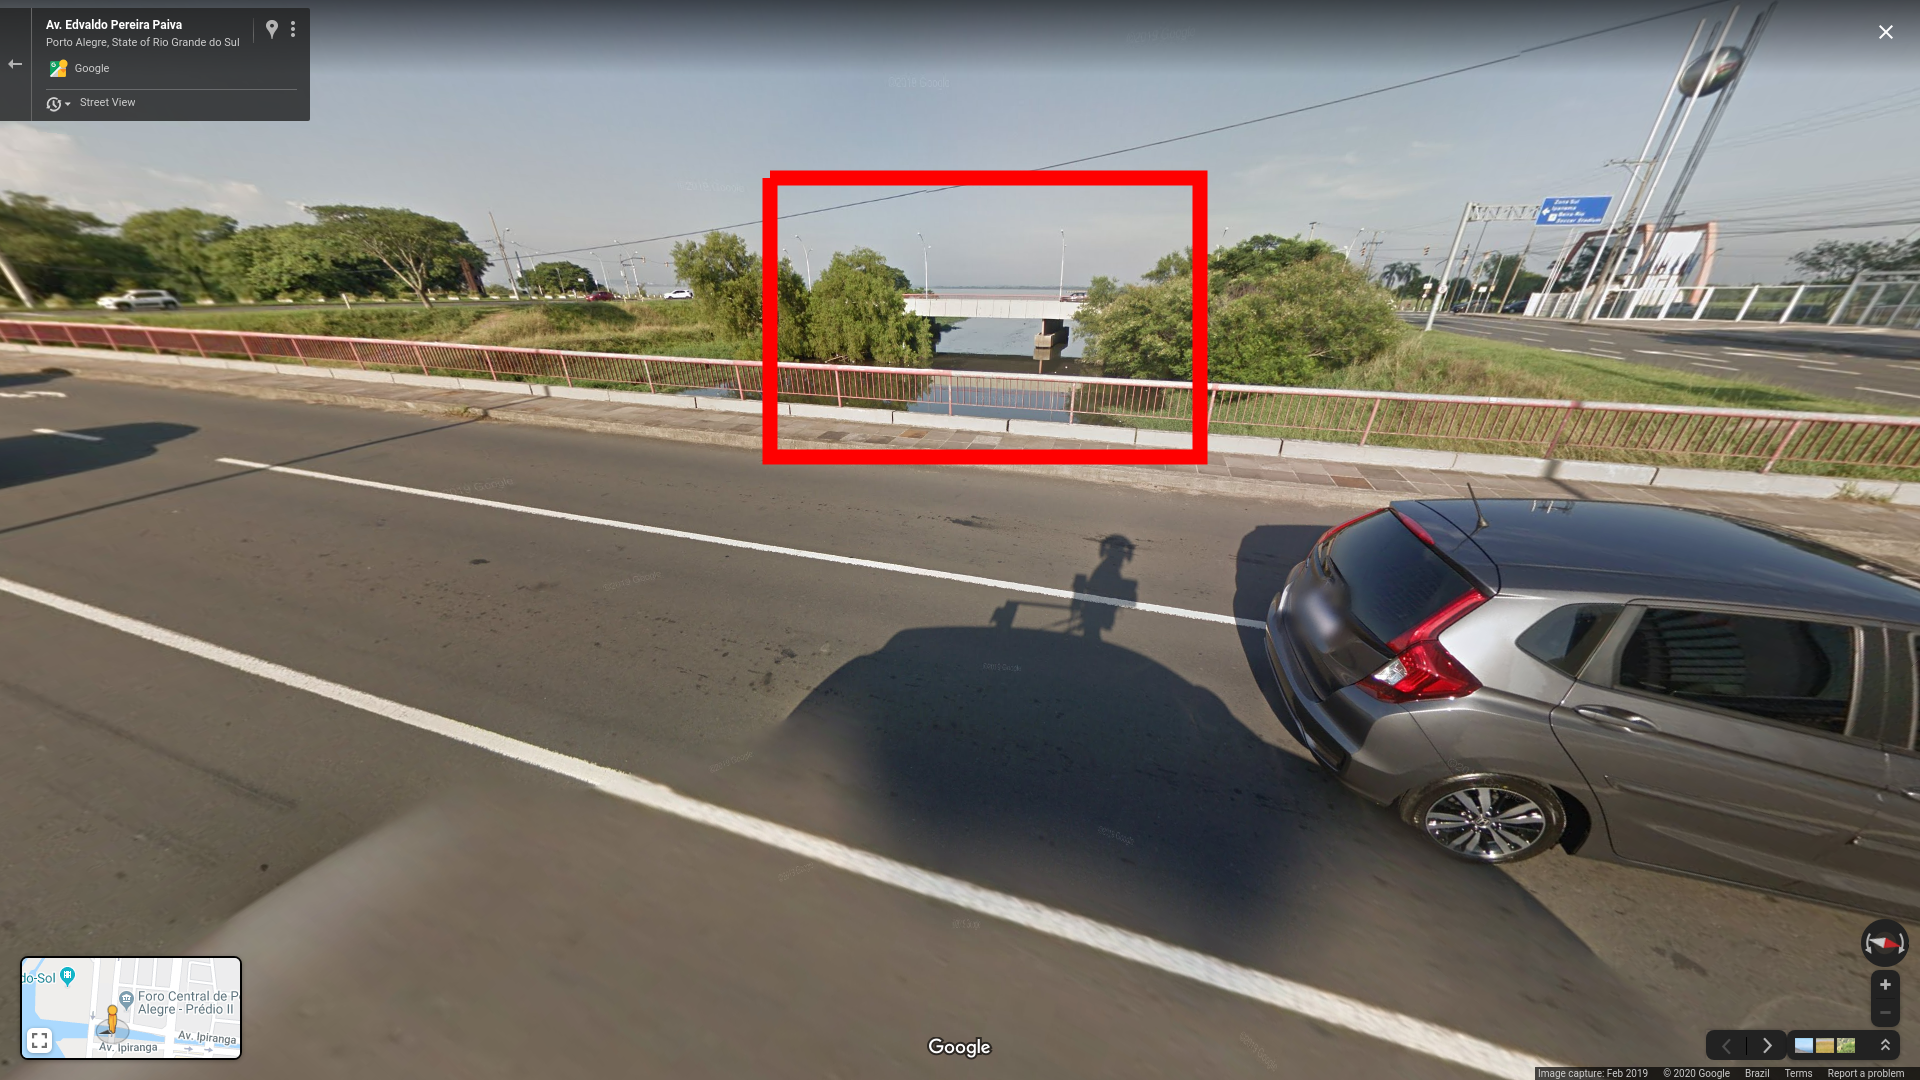
\includegraphics[scale=0.1]{figs/simulation_diluvio_googleLocation2_1_roundedArea.png}
            \caption{Real World}
            \label{fig:simulation_diluvio_googleLocation2_1_roundedArea}
        \end{subfigure}
        \begin{subfigure}[b]{0.4\textwidth}
            \centering
            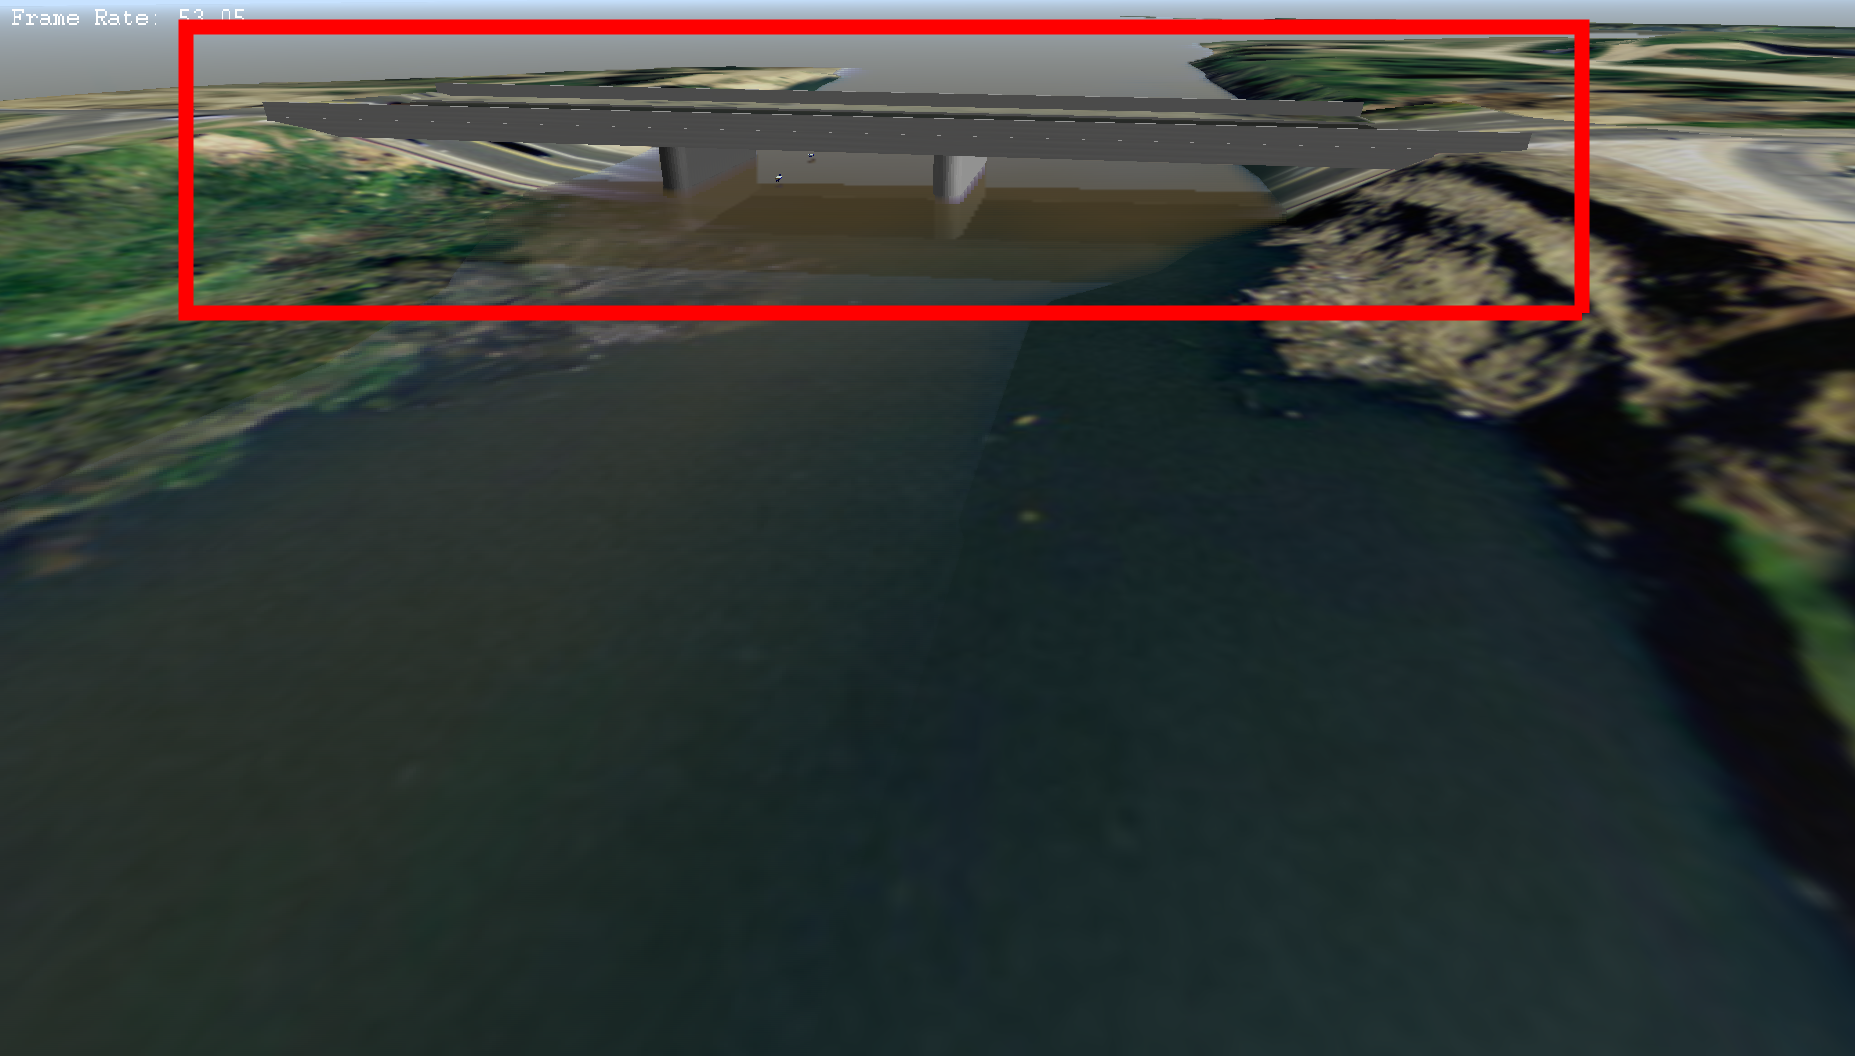
\includegraphics[scale=0.1]{figs/simulation_diluvio_googleLocation2_2_roundedArea.png}
            \caption{Real World Simulated}
            \label{fig:simulation_diluvio_googleLocation2_2_roundedArea}
        \end{subfigure}
    
    \caption{Real world region and its simulated version}
    \label{fig:simulation_diluvio_googleLocation2_roundedArea}
    \end{figure}
    
    % As presented in Chapter \ref{chap:2_TheoreticalBackground}, a head-on scenario is mainly characterized by an encounter between two vessels with a relative bearing of 30°. The assembled scenario is presented in Figure \ref{fig:simulation_uwsim_encounters}.
    
    \begin{figure}[H]
    \centering
    
        \begin{subfigure}[b]{0.5\textwidth}
            \centering
            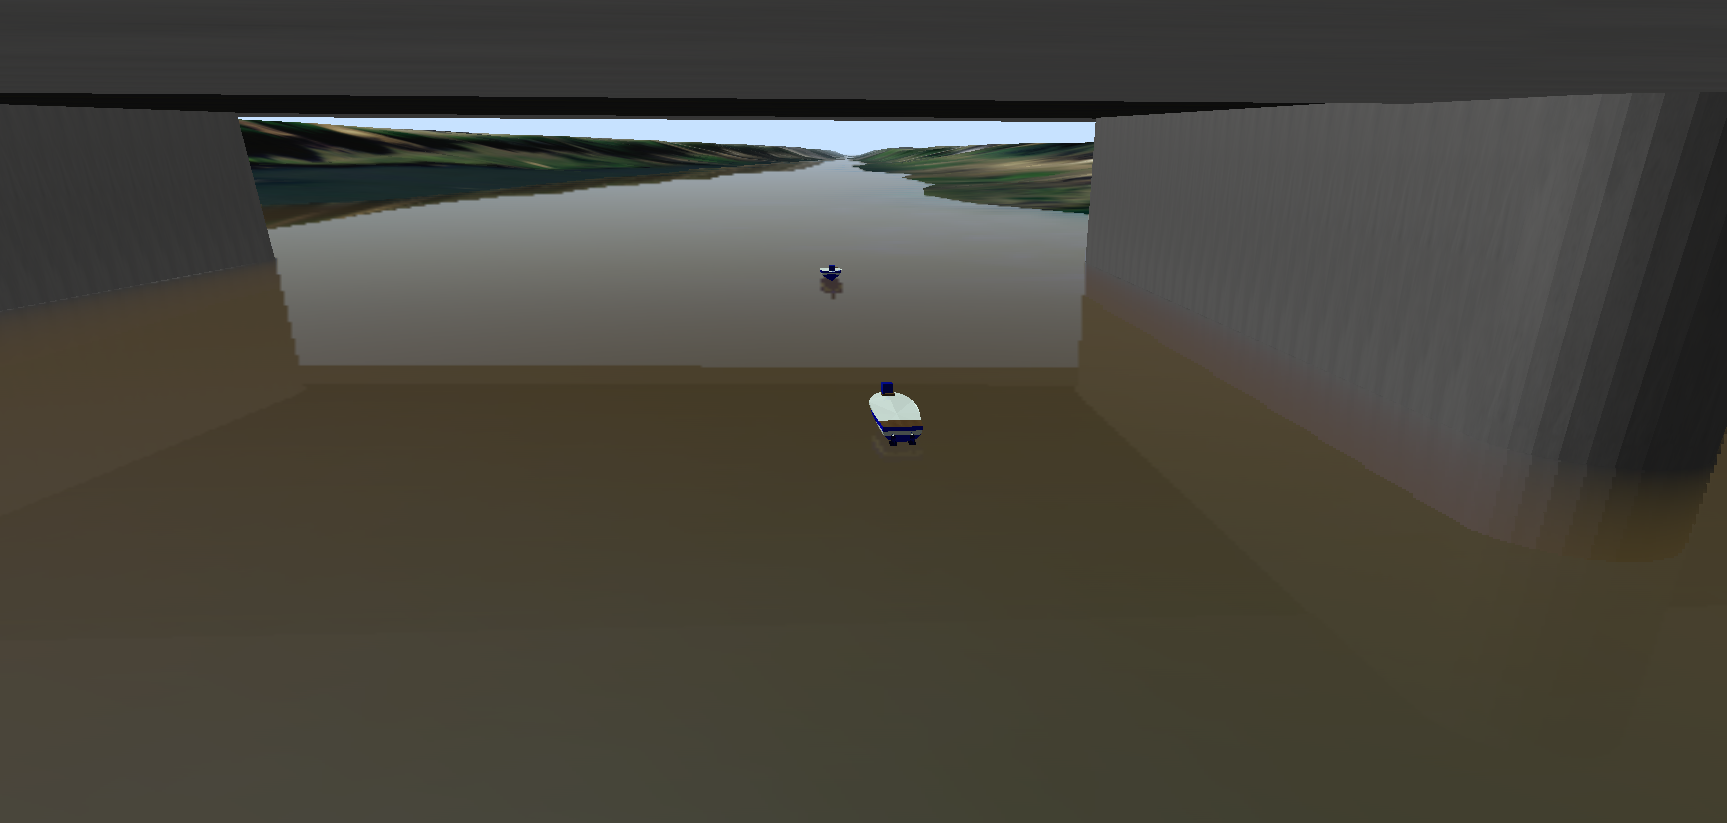
\includegraphics[width=\textwidth]{figs/simulation_uwsim_headon_starting_pos.png}
            \caption{Head On}
            \label{fig:simulation_uwsim_headon_starting_pos}
        \end{subfigure}
        \begin{subfigure}[b]{0.45\textwidth}
            \centering
            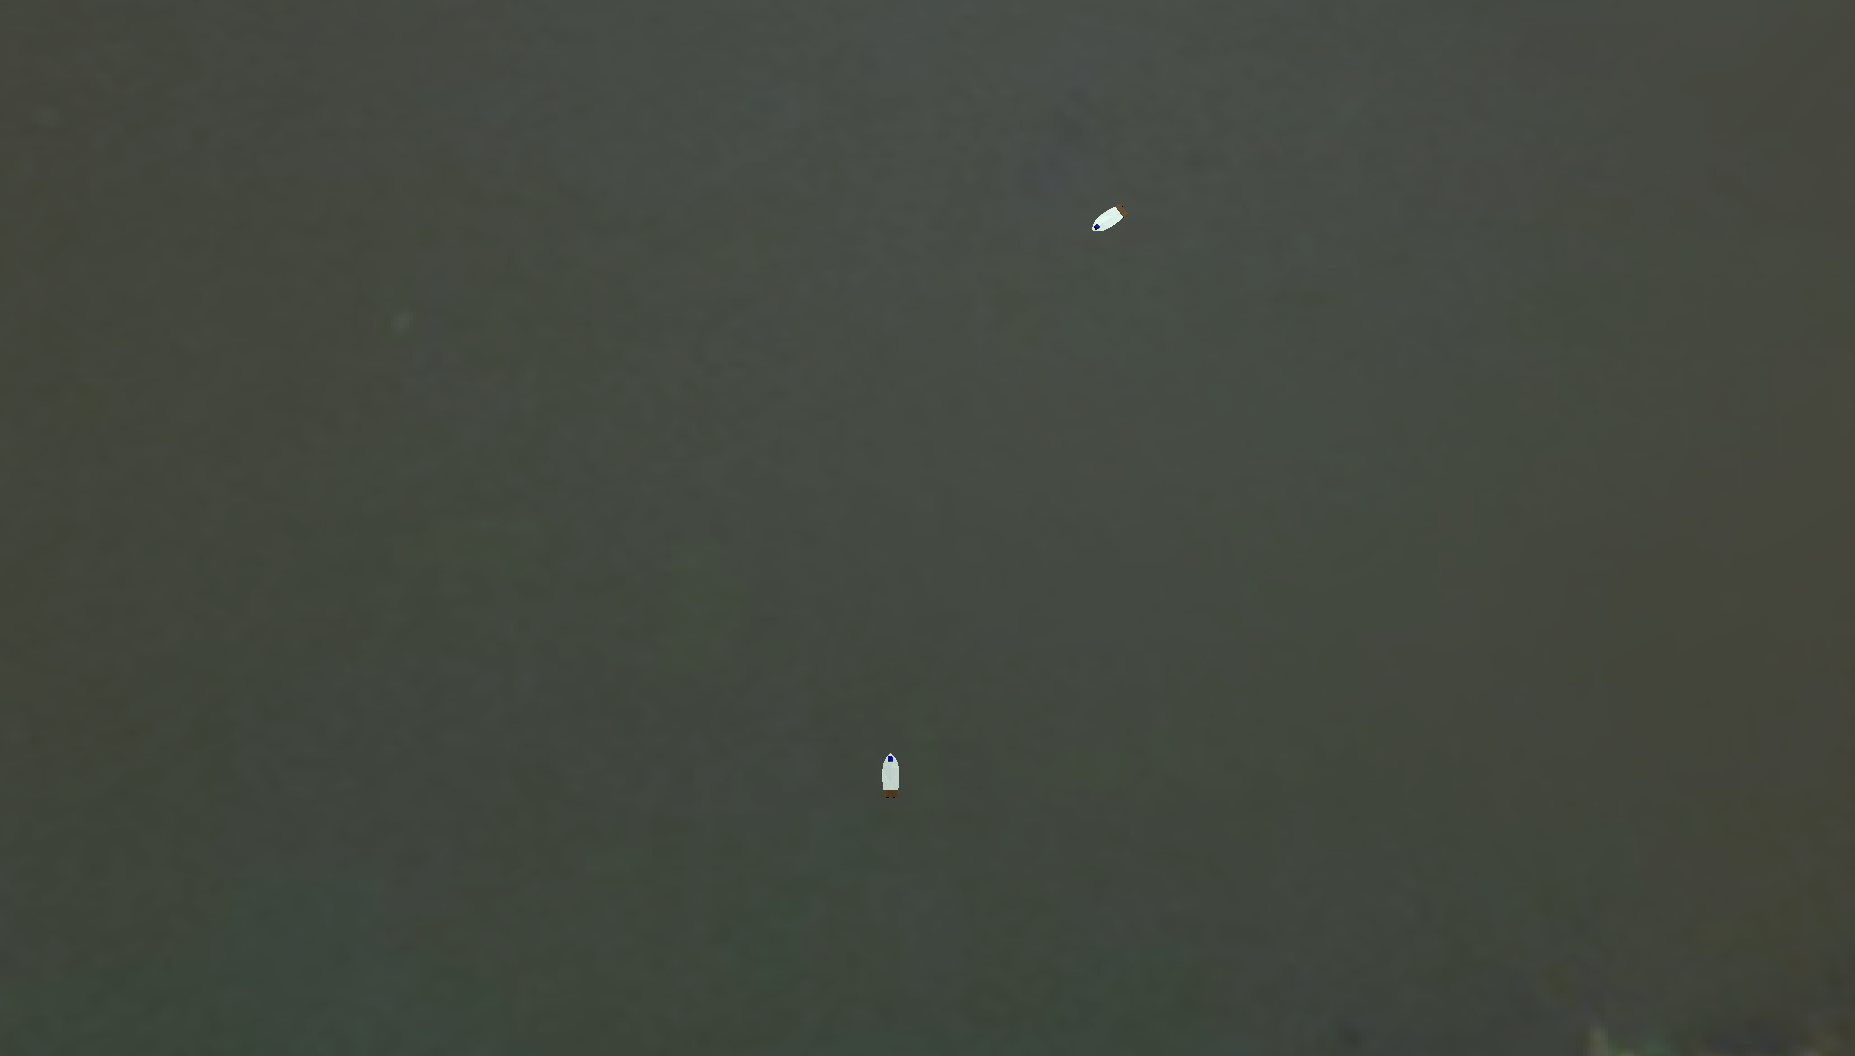
\includegraphics[width=\textwidth]{figs/simulation_uwsim_crossingright_starting_pos.png}
            \caption{Crossing from Right}
            \label{fig:simulation_uwsim_crossingright_starting_pos}
        \end{subfigure}
        
        \begin{subfigure}[b]{0.5\textwidth}
            \centering
            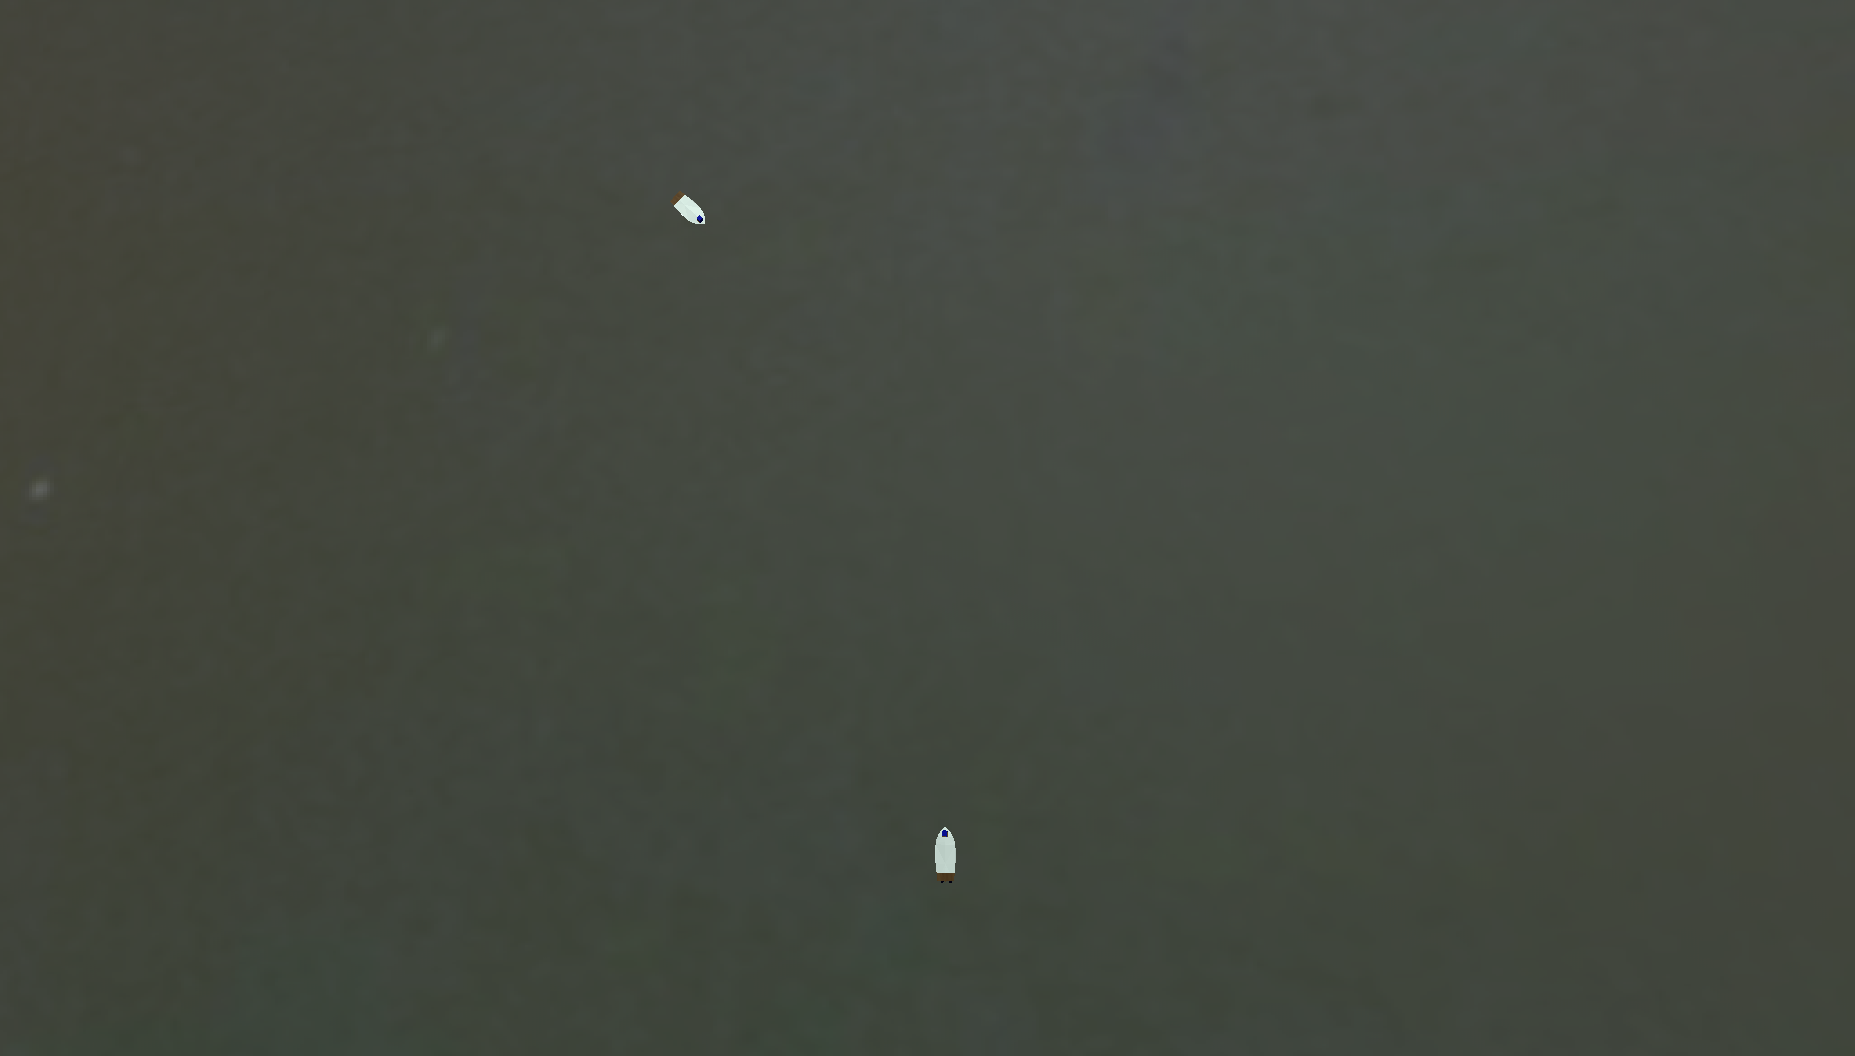
\includegraphics[width=\textwidth]{figs/simulation_uwsim_crossingleft_starting_pos.png}
            \caption{Crossing from Left}
            \label{fig:simulation_uwsim_crossingleft_starting_pos}
        \end{subfigure}
        \begin{subfigure}[b]{0.45\textwidth}
            \centering
            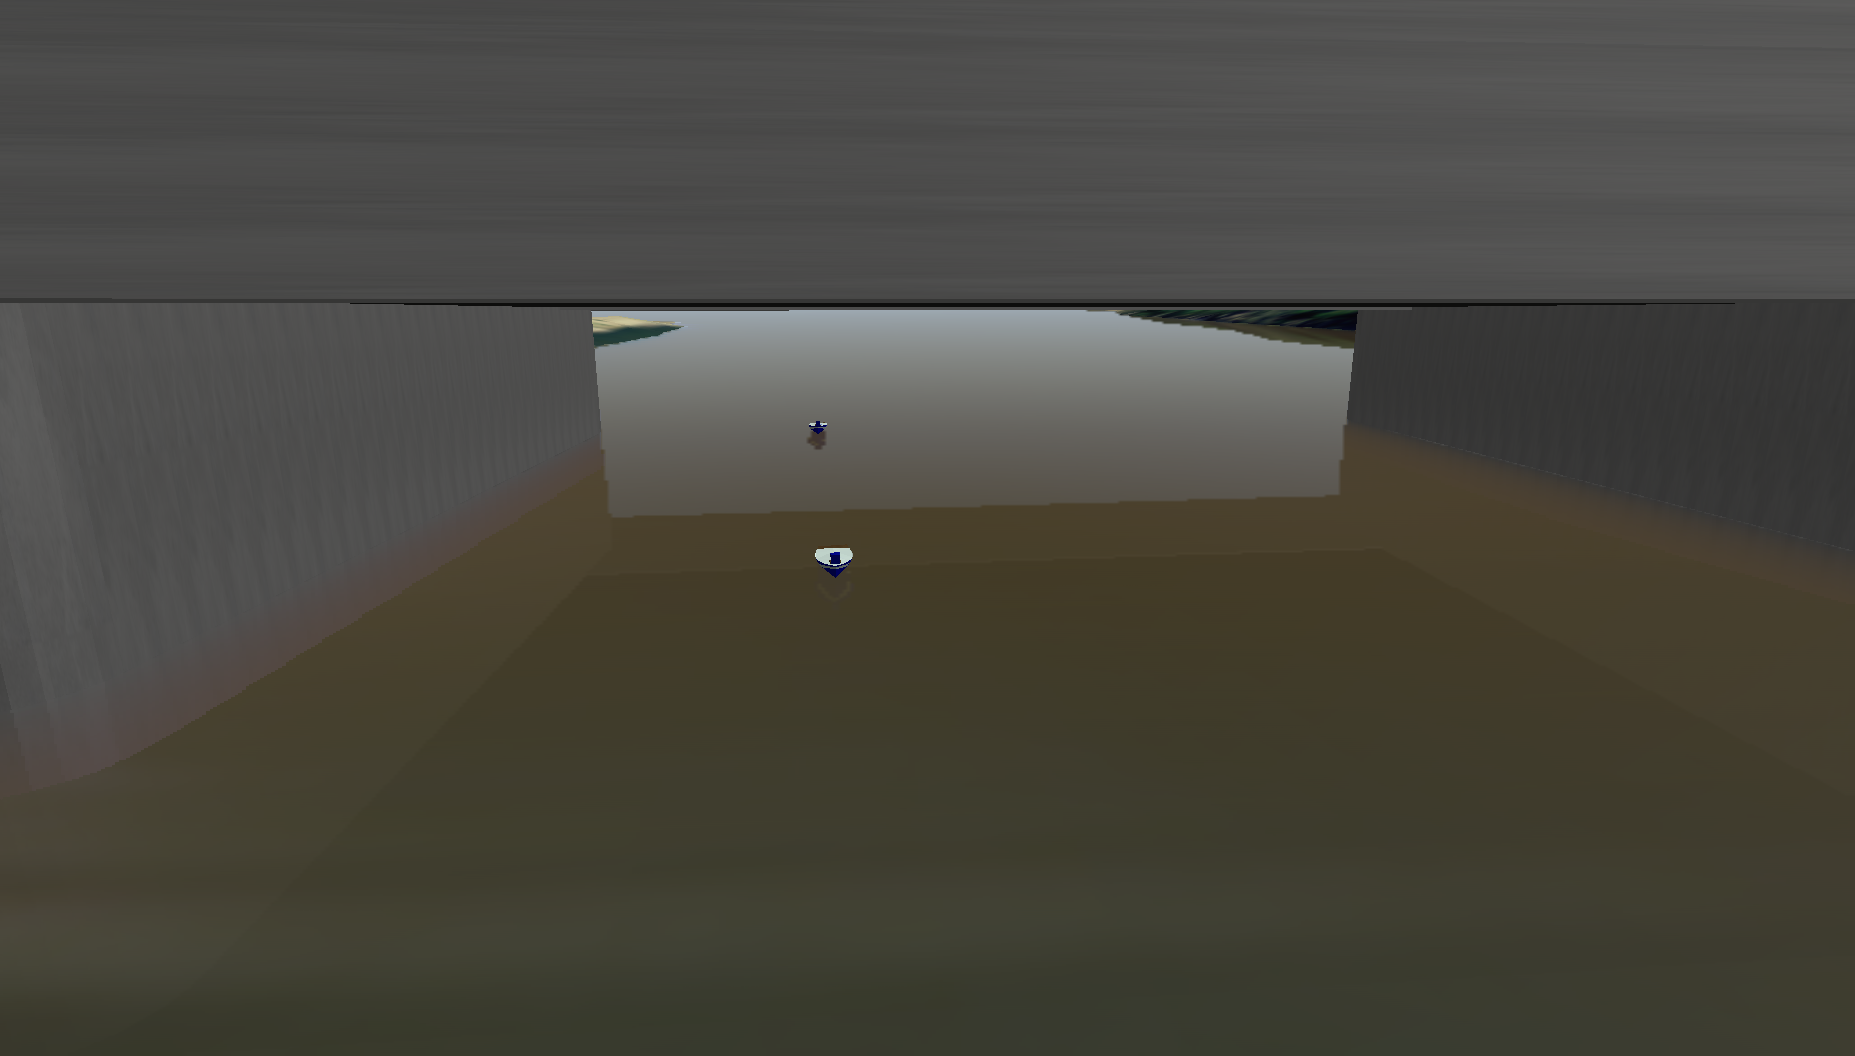
\includegraphics[width=\textwidth]{figs/simulation_uwsim_overtake_starting_pos.png}
            \caption{Overtaking}
            \label{fig:simulation_uwsim_overtake_starting_pos}
        \end{subfigure}
    
    \caption{Encounter scenarios for evaluation. Scenarios adopted from ~\cite{Huang2019Generalized}.}
    \label{fig:simulation_uwsim_encounters}
    \end{figure}

%AMA a figura dos barcos esta muito pequena. veja como fica na versao impressa. acho q vc vai ter q pelo menos desenhar uma flecha p indicar a direcao dos barcos.

    \begin{center}
        \savebox{\mytablebox}{\begin{tabular}{cccc}
        
        \toprule[3pt]
        \multicolumn{4}{c}{\textbf{Own Vessel}} \\
        \midrule
        \textbf{Encounter Type} & \textbf{Initial Pose (m, m, º)} & \textbf{Target Position} &  \textbf{Max. Speed (m/s)}\\
        \midrule
        Head On &  (450, 107.5, 0)  &   (480, 107.5)   &  0.4 \\
        Crossing Right &  (410, 105, 90)  &  (410, 133)   &  0.86  \\
        Crossing Left &  (410, 105, 90)  & (410, 133)   &  0.29  \\
        Overtaking &  (450, 107.5, 0)  &  (550, 107.5)   &  0.5 \\
        \bottomrule
        
        \end{tabular}}
        \settowidth{\mytablewidth}{\usebox{\mytablebox}}
        \begin{minipage}{\mytablewidth}
        \captionof{table}{Encounter Scenarios Configuration - Own Vessel}
        \label{tab:simulation_scenarios_configuration_own_vessel}
        \usebox{\mytablebox}
        \end{minipage}

    \end{center}
    
    \begin{center}
        \savebox{\mytablebox}{\begin{tabular}{cccc}
        
        \toprule[3pt]
        \multicolumn{4}{c}{\textbf{Encountering Vessel}} \\
        \midrule
        \textbf{Encounter Type} & \textbf{Initial Pose (m, m, º)} & \textbf{Target Position} & \textbf{Max. Speed (m/s)}\\
        \midrule
        Head On &  (450, 107.5, 0)  &   (480, 107.5)   &  0.4 \\
        Crossing Right &  (410, 105, 90)  &  (410, 133)   &  0.86  \\
        Crossing Left &  (410, 105, 90)  & (410, 133)   &  0.29  \\
        Overtaking &  (450, 107.5, 0)  &  (550, 107.5)   &  0.5 \\
        \bottomrule
        
        \end{tabular}}
        \settowidth{\mytablewidth}{\usebox{\mytablebox}}
        \begin{minipage}{\mytablewidth}
        \captionof{table}{Encounter Scenarios Configuration - Encountering Vessel}
        \label{tab:simulation_scenarios_configuration_encountering_vessel}
        \usebox{\mytablebox}
        \end{minipage}

    \end{center}

%AMA a apresentacao da tabela está realmente feia ! Latex tem formatos bem legais. Sugiro melhorar esse aspecto. Tb sugiro fortemente colocar na fig anterior o local do initial pose, destination, e trajetoria. Acho q deve trocar Waypoint por destination ou target position.
%DJ: Done
    
    \section{Experiments Results}
    
        % Grammarlly: 100/100
        We adopted scientific experimentation for \ac{ATC} correctness validation, running the same scenario twice, one execution with \ac{ATC}, and another without \ac{ATC}. Results and their respective description for head-on, crossing from right, crossing from left and overtaking scenarios are presented respectively in Figures \ref{fig:headOn_E}, \ref{fig:crossingRight_E}, \ref{fig:crossingLeft_E} and \ref{fig:overtaking_E}. For each scenario, we measured the computation time of every execution of our path planner, average sustained speed, and minimal distance maintained between the vessels, and evaluated successful avoidance. In Table \ref{tab:results} we show collected results.
        
        \begin{figure}[H]
        \centering
        
            \begin{subfigure}[b]{0.45\textwidth}
                \centering
                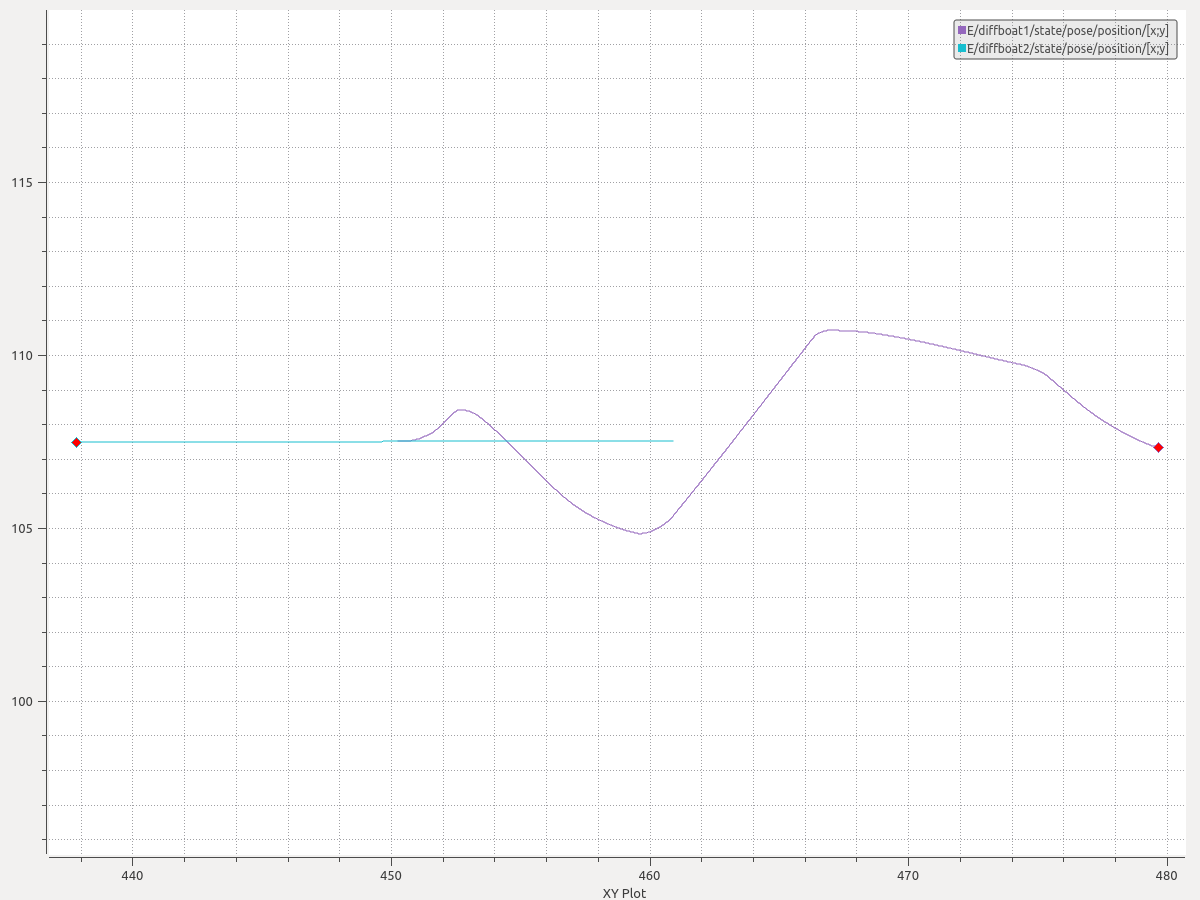
\includegraphics[width=\textwidth]{figs/plot_headOn_E.png}
                \caption{With \ac{ATC}}
                \label{fig:plot_headOn_E}
            \end{subfigure}
            \begin{subfigure}[b]{0.45\textwidth}
                \centering
                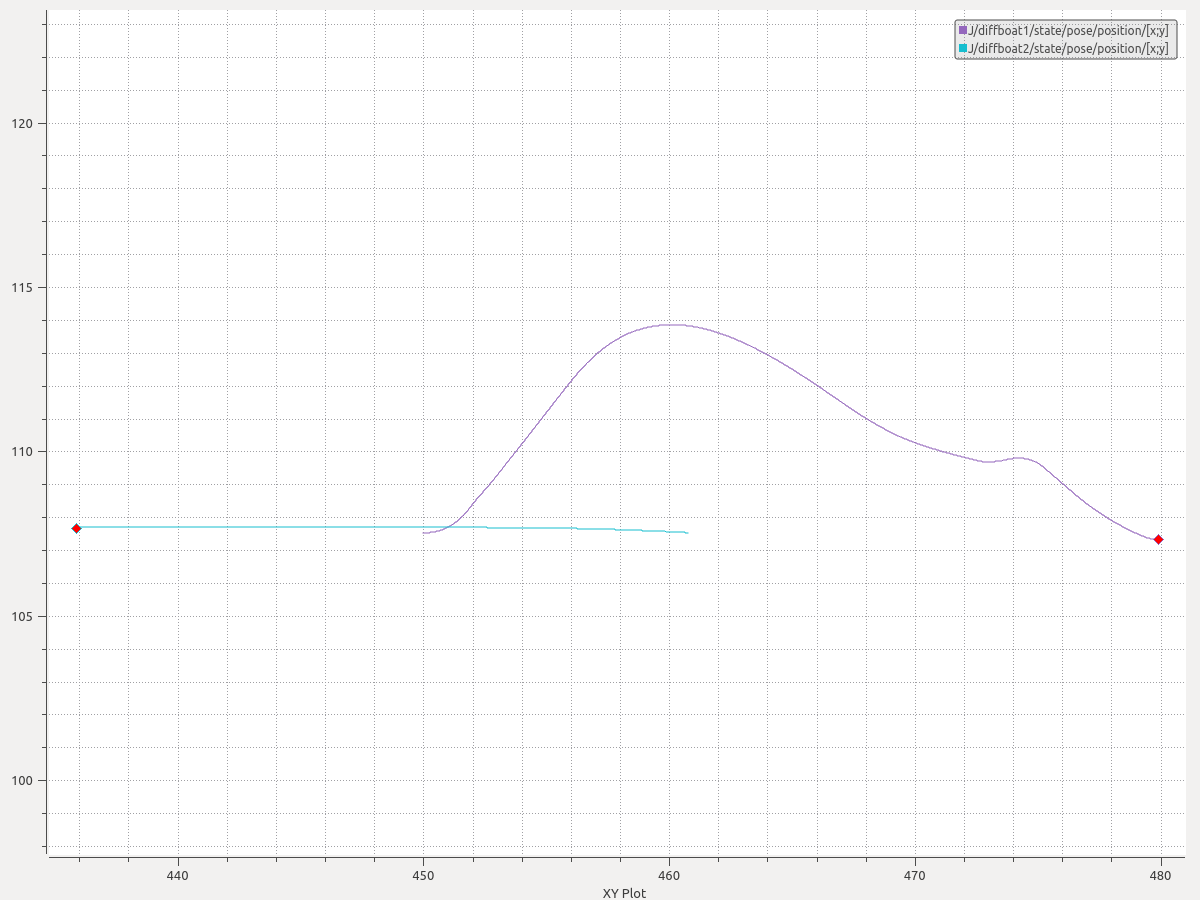
\includegraphics[width=\textwidth]{figs/plot_noATC_headOn_E.png}
                \caption{Without \ac{ATC}}
                \label{fig:plot_noATC_headOn_E}
            \end{subfigure}
            
            \begin{subfigure}[b]{0.45\textwidth}
                \centering
                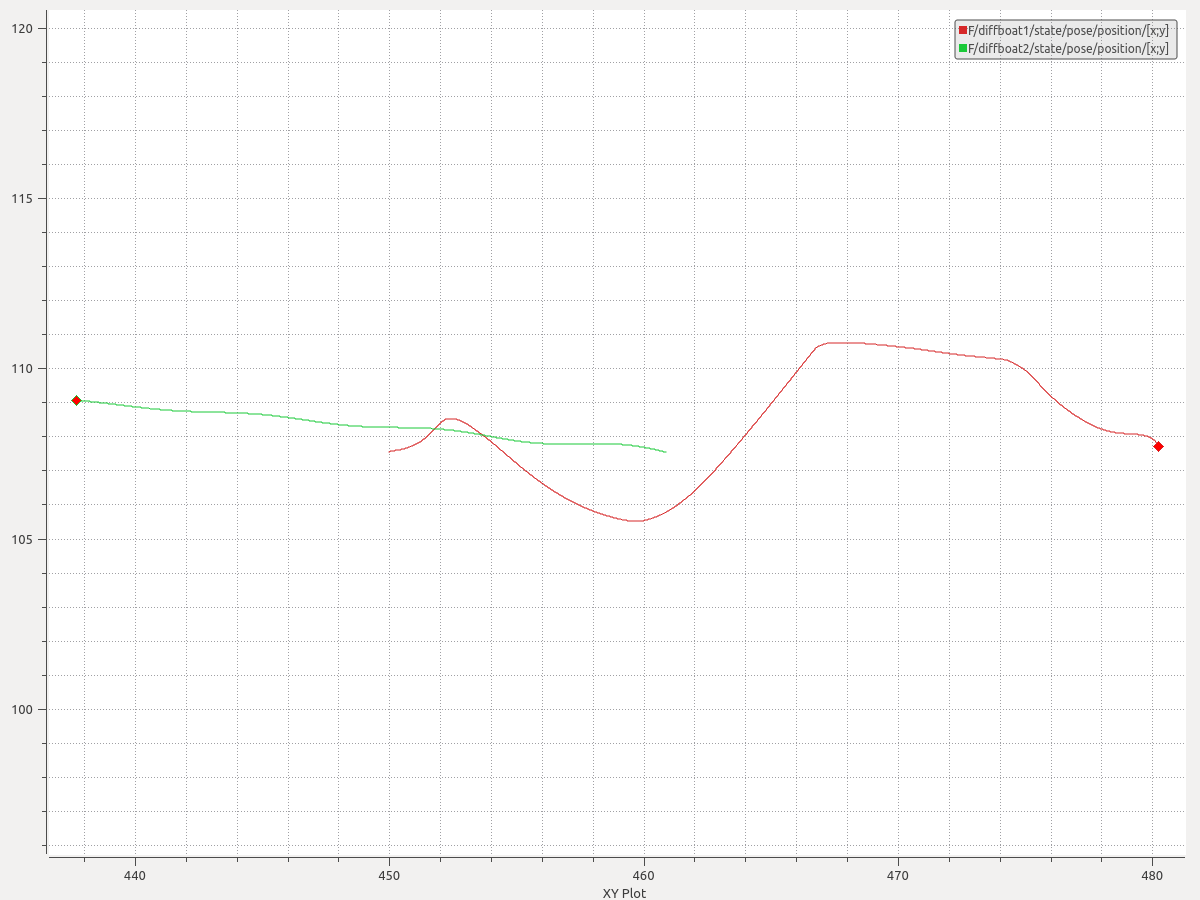
\includegraphics[width=\textwidth]{figs/plot_headOn_Wind_E.png}
                \caption{With \ac{ATC} and Wind}
                \label{fig:plot_headOn_Wind_E}
            \end{subfigure}
            % \begin{subfigure}[b]{0.45\textwidth}
            %     \centering
            %     \includegraphics[width=\textwidth]{figs/plot_Overtaking_Wind_BAD_E.png}
            %     \caption{\ac{ATC} and Bad Wind}
            %     \label{fig:plot_headOn_Wind__BAD_E}
            % \end{subfigure}
        
        \caption{DESCRIÇÂO DOS GRAFICOS AQUI: }
        \label{fig:headOn_E}
        \end{figure}
%AMA a legenda dass trajetorias esta ilegivel. ou vc aumenta ate ficar legivel ou remove dali. se remover, vc pode descrever o significado das cores na legenda.
%AMA do jeito q está, nao eh facil comparar um grafico c o outro. seria MUITO melhor se vc conseguir colocar dois plots juntos. por exemplo, with ATC e wo/ ATC. with ATC e with ATC + wind. Nao junta os 3 pois acho q vai poluir demais.
% AMA a legenda dos eixos tb nao deve estar legivel p impressao. aumente o texto dos nros.
%AMA o ponto vermelho eh o ponto inicial ou final. deixar isso claro na legenda
%AMA qnd tiver vento, anota na figura a dirececao e velocidade tb.
        
         \begin{figure}[H]
        \centering
        
            \begin{subfigure}[b]{0.45\textwidth}
                \centering
                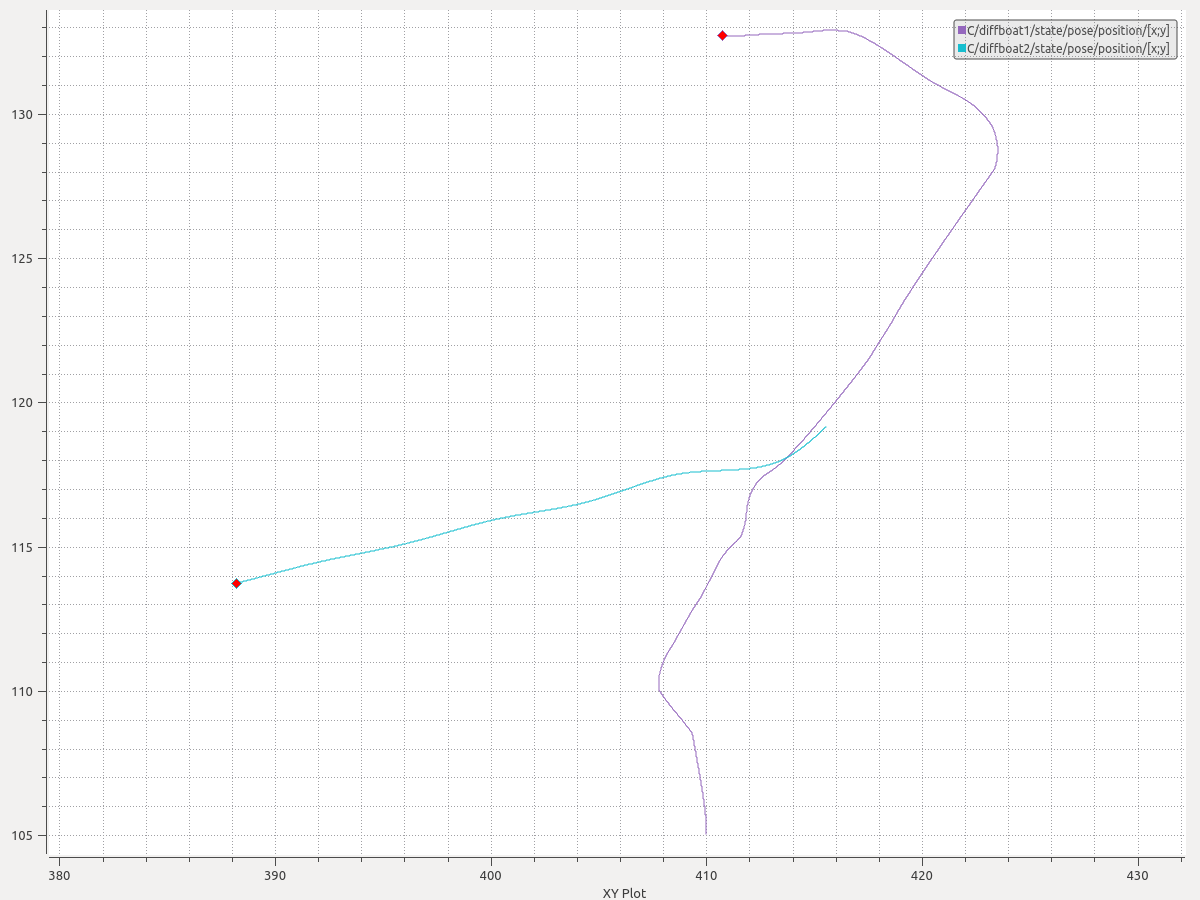
\includegraphics[width=\textwidth]{figs/plot_crossingRight_E.png}
                \caption{With \ac{ATC}}
                \label{fig:plot_crossingRight_E}
            \end{subfigure}
            \begin{subfigure}[b]{0.45\textwidth}
                \centering
                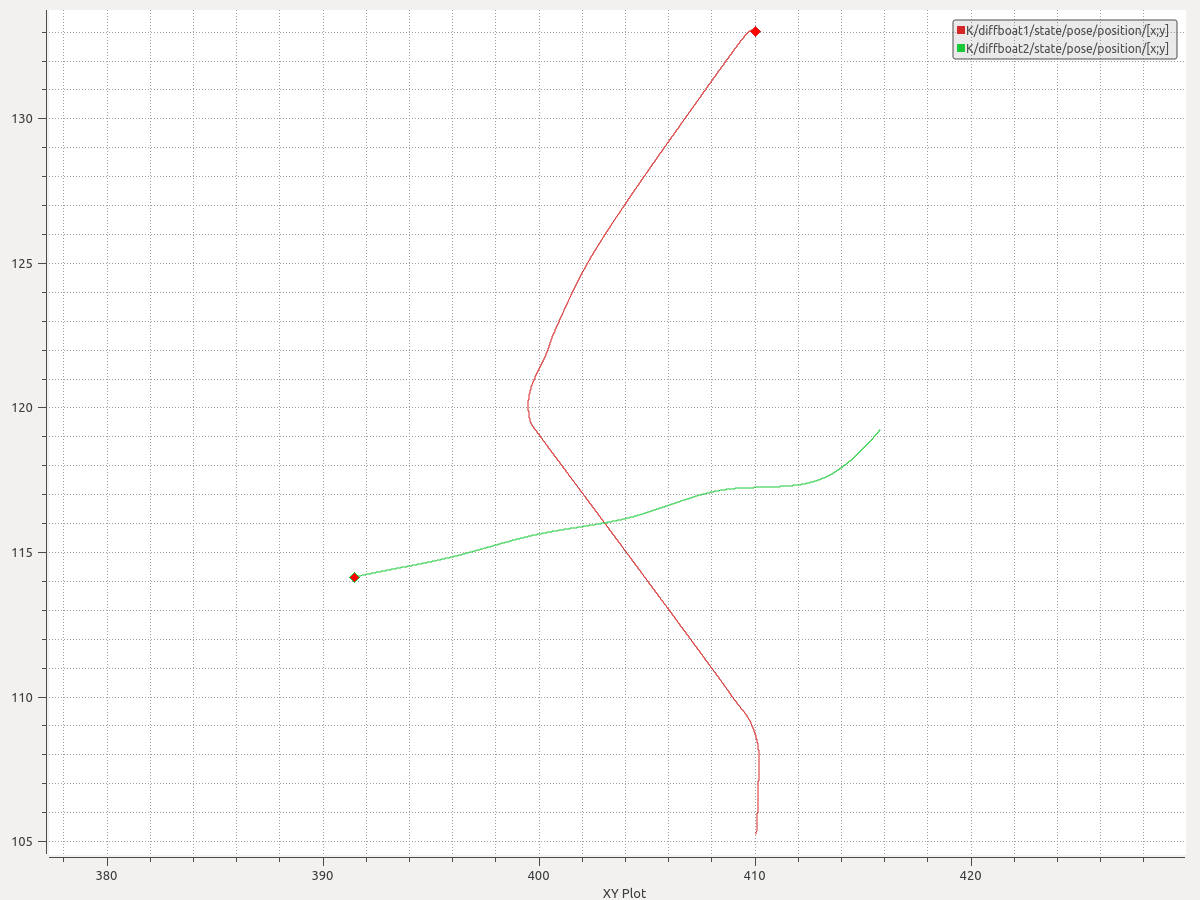
\includegraphics[width=\textwidth]{figs/plot_noATC_crossingRight_E.png}
                \caption{Without \ac{ATC}}
                \label{fig:plot_noATC_crossingRight_E}
            \end{subfigure}
            
            \begin{subfigure}[b]{0.45\textwidth}
                \centering
                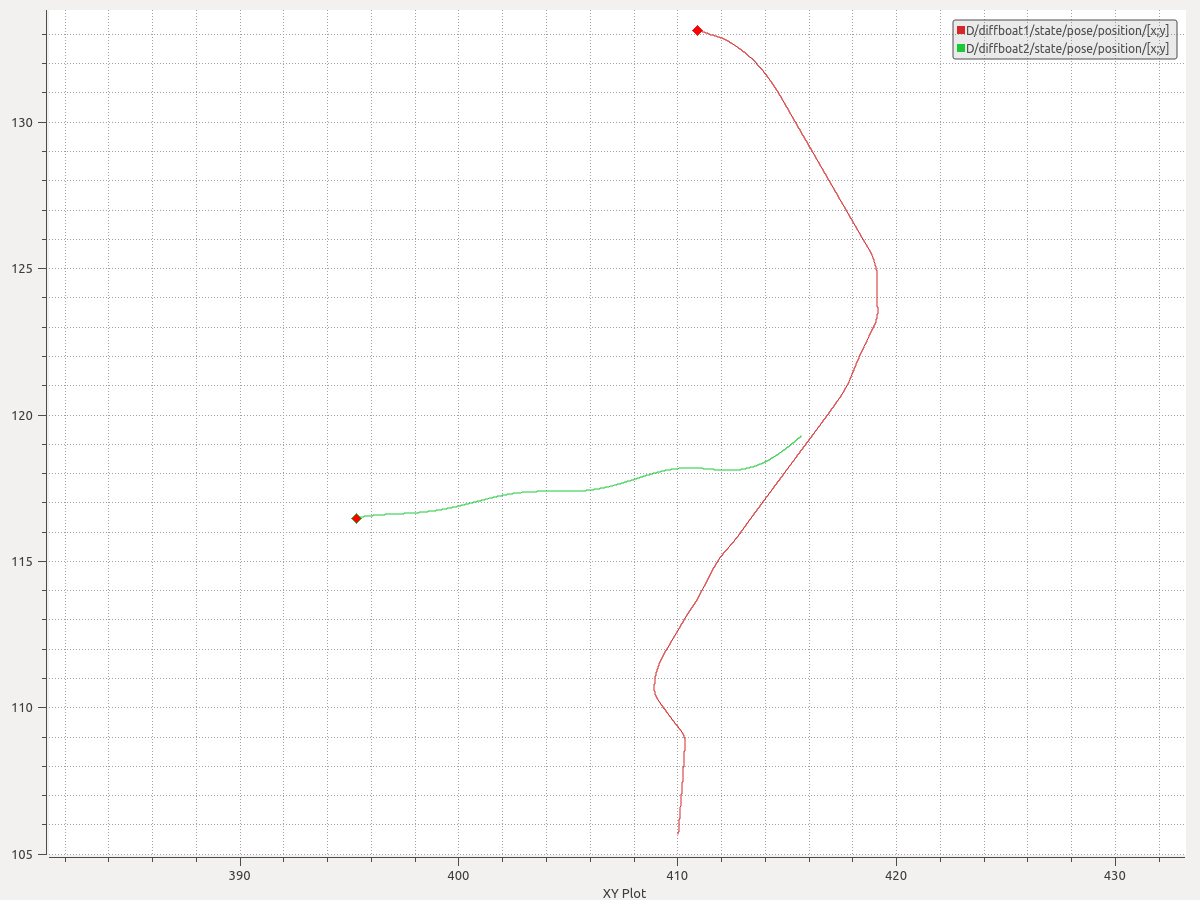
\includegraphics[width=\textwidth]{figs/plot_crossingRight_Wind_E.png}
                \caption{With \ac{ATC} and Wind}
                \label{fig:plot_crossingRight_Wind_E}
            \end{subfigure}
            % \begin{subfigure}[b]{0.45\textwidth}
            %     \centering
            %     \includegraphics[width=\textwidth]{figs/plot_Overtaking_Wind_BAD_E.png}
            %     \caption{\ac{ATC} and Bad Wind}
            %     \label{fig:plot_crossingRight_Wind__BAD_E}
            % \end{subfigure}
        
        \caption{DESCRIÇÂO DOS GRAFICOS AQUI: }
        \label{fig:crossingRight_E}
        \end{figure}
        
         \begin{figure}[H]
        \centering
        
            \begin{subfigure}[b]{0.45\textwidth}
                \centering
                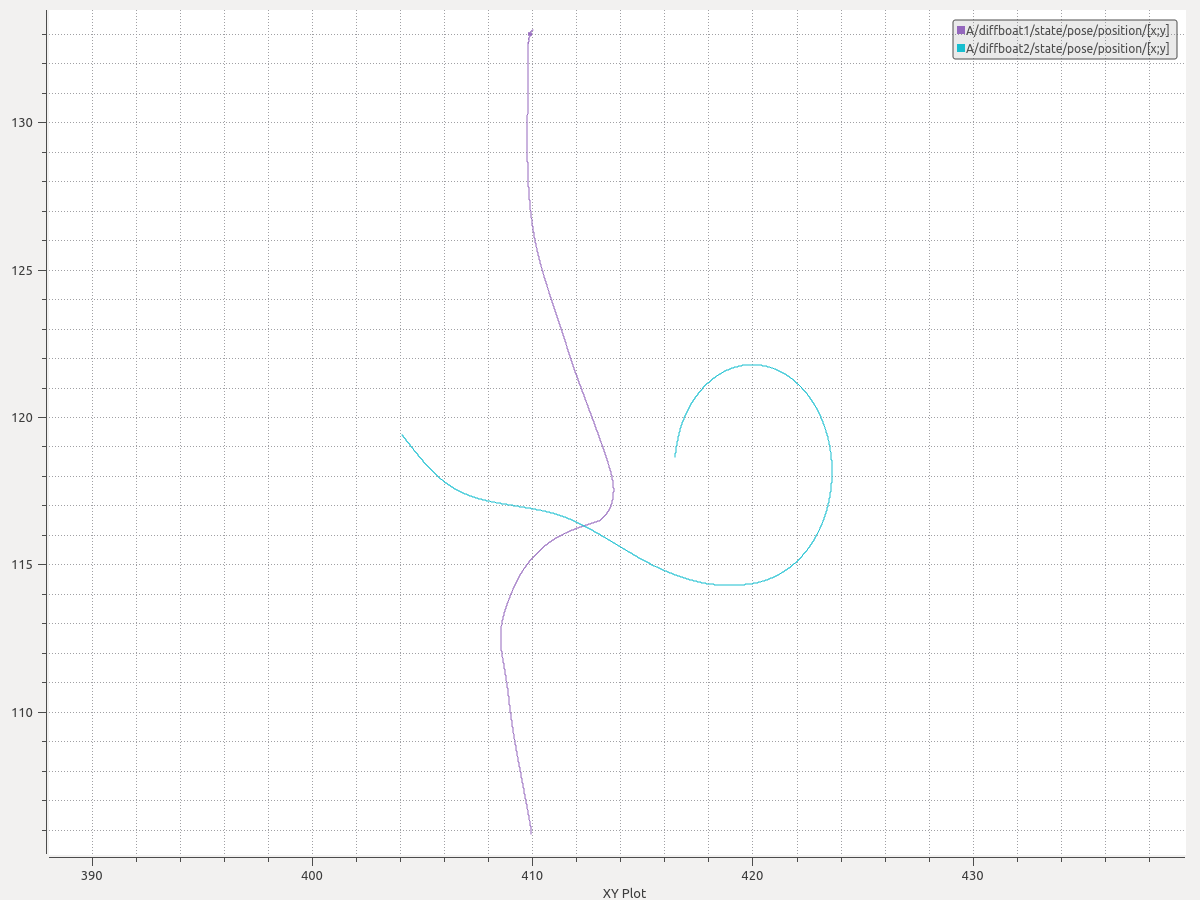
\includegraphics[width=\textwidth]{figs/plot_crossingLeft_E.png}
                \caption{With \ac{ATC}}
                \label{fig:plot_crossingLeft_E}
            \end{subfigure}
            \begin{subfigure}[b]{0.45\textwidth}
                \centering
                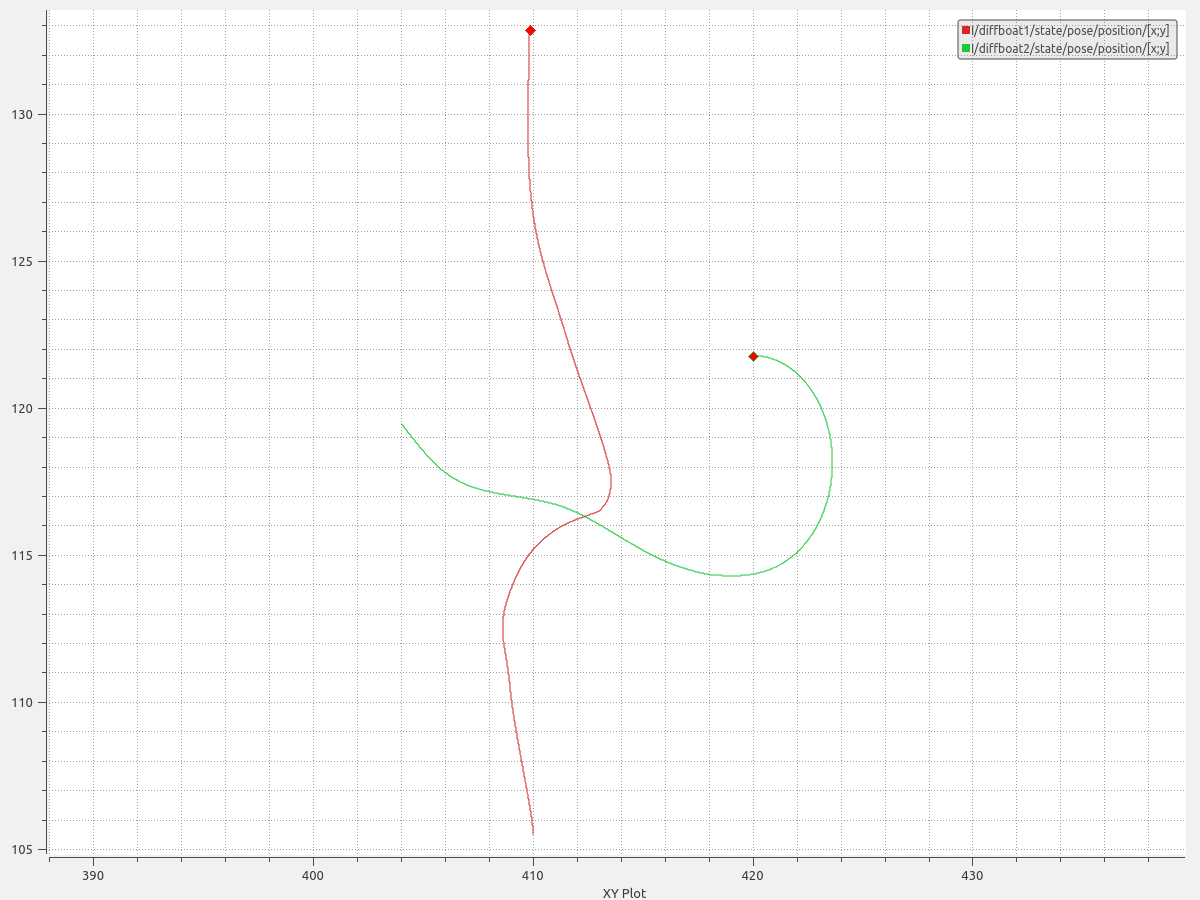
\includegraphics[width=\textwidth]{figs/plot_noATC_crossingLeft_E.png}
                \caption{Without \ac{ATC}}
                \label{fig:plot_noATC_crossingLeft_E}
            \end{subfigure}
            
            \begin{subfigure}[b]{0.45\textwidth}
                \centering
                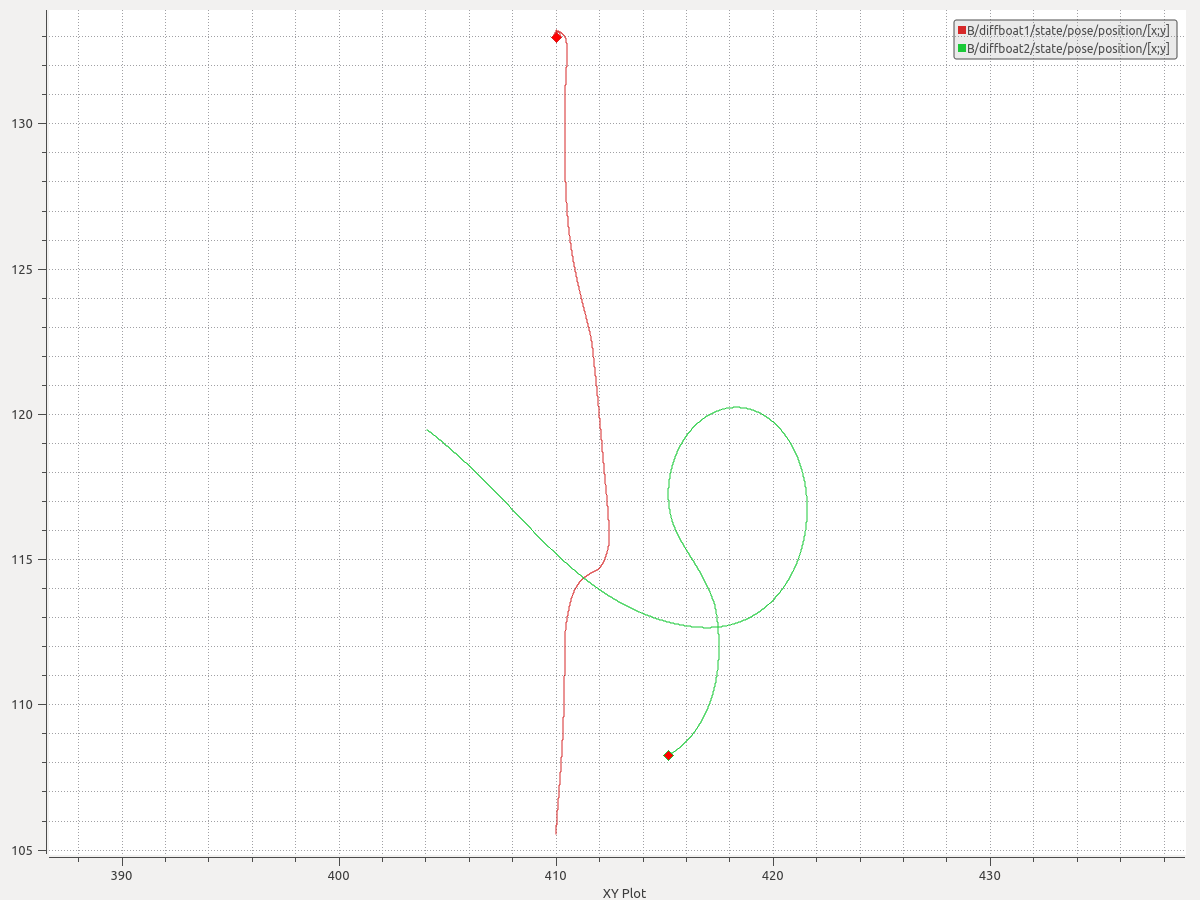
\includegraphics[width=\textwidth]{figs/plot_crossingLeft_Wind_E.png}
                \caption{With \ac{ATC} and Wind}
                \label{fig:plot_crossingLeft_Wind_E}
            \end{subfigure}
            % \begin{subfigure}[b]{0.45\textwidth}
            %     \centering
            %     \includegraphics[width=\textwidth]{figs/plot_Overtaking_Wind_BAD_E.png}
            %     \caption{\ac{ATC} and Bad Wind}
            %     \label{fig:plot_crossingLeft_Wind__BAD_E}
            % \end{subfigure}
        
        \caption{DESCRIÇÂO DOS GRAFICOS AQUI: Crossing Left Encounter}
        \label{fig:crossingLeft_E}
        \end{figure}
        
         \begin{figure}[H]
        \centering
        
            \begin{subfigure}[b]{0.45\textwidth}
                \centering
                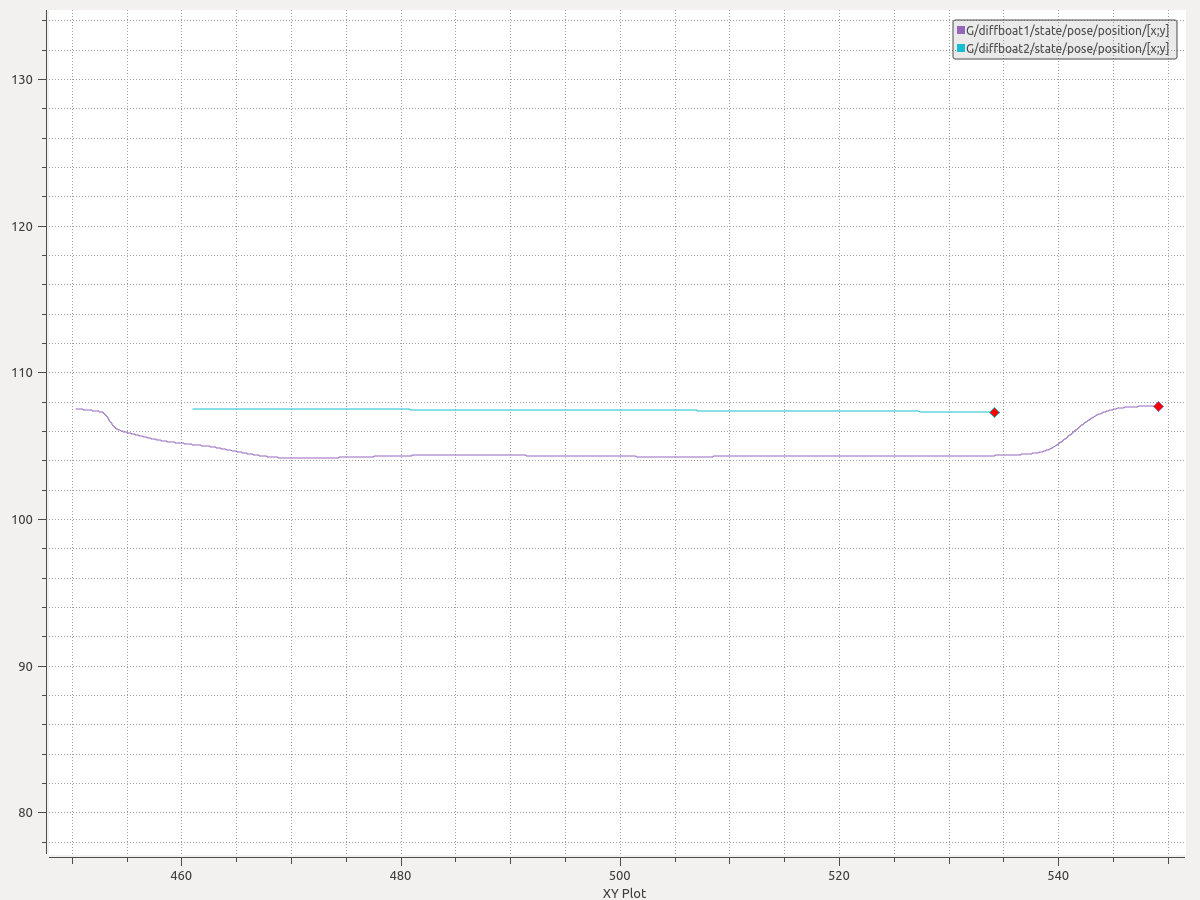
\includegraphics[width=\textwidth]{figs/plot_overtaking_E.png}
                \caption{With \ac{ATC}}
                \label{fig:plot_overtaking_E}
            \end{subfigure}
            \begin{subfigure}[b]{0.45\textwidth}
                \centering
                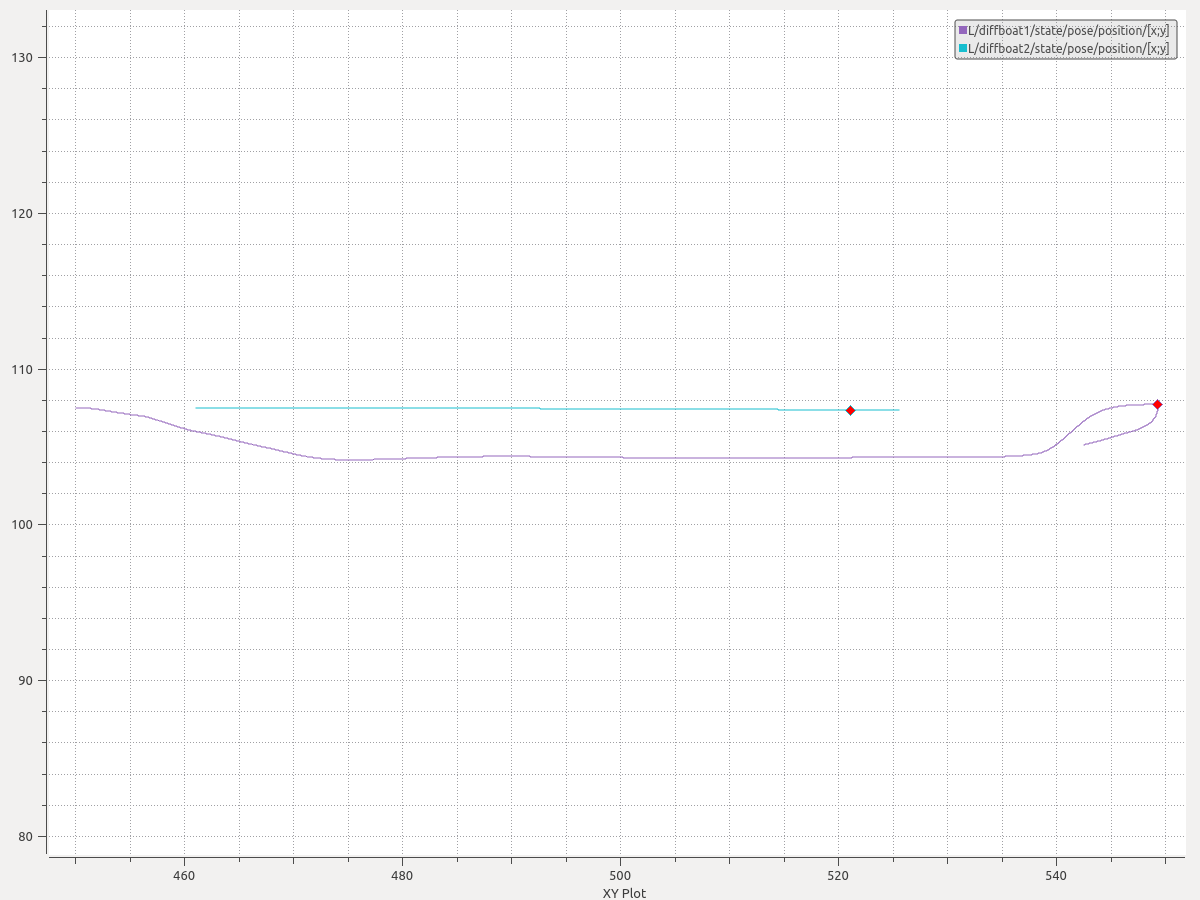
\includegraphics[width=\textwidth]{figs/plot_noATC_overtaking_E.png}
                \caption{Without \ac{ATC}}
                \label{fig:plot_noATC_overtaking_E}
            \end{subfigure}
            
            \begin{subfigure}[b]{0.45\textwidth}
                \centering
                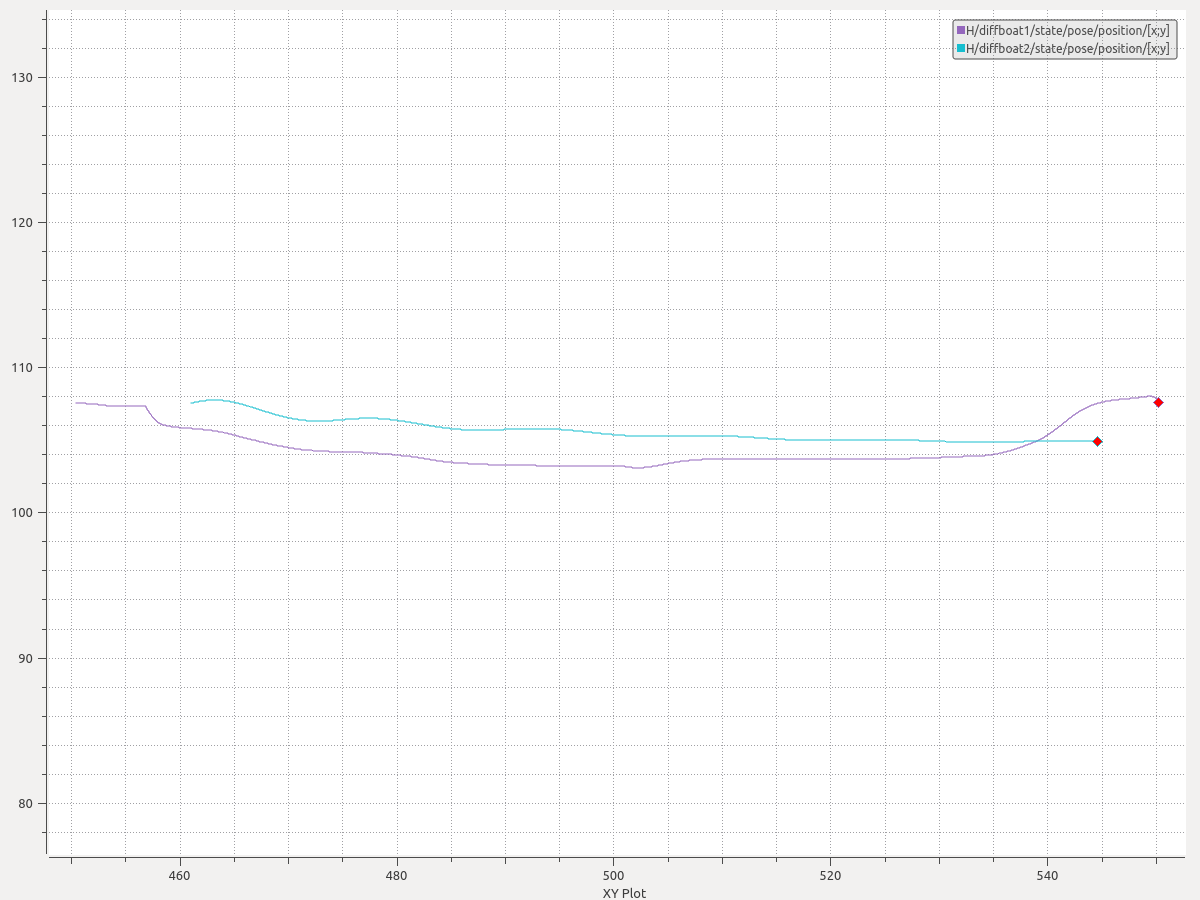
\includegraphics[width=\textwidth]{figs/plot_overtaking_Wind_E.png}
                \caption{With \ac{ATC} and Wind}
                \label{fig:plot_overtaking_Wind_E}
            \end{subfigure}
            % \begin{subfigure}[b]{0.45\textwidth}
            %     \centering
            %     \includegraphics[width=\textwidth]{figs/plot_Overtaking_Wind_BAD_E.png}
            %     \caption{\ac{ATC} and Bad Wind}
            %     \label{fig:plot_overtaking_Wind__BAD_E}
            % \end{subfigure}
        
        \caption{DESCRIÇÂO DOS GRAFICOS AQUI: }
        \label{fig:overtaking_E}
        \end{figure}

        
        % \begin{figure}[H]
        %     \centering
        %     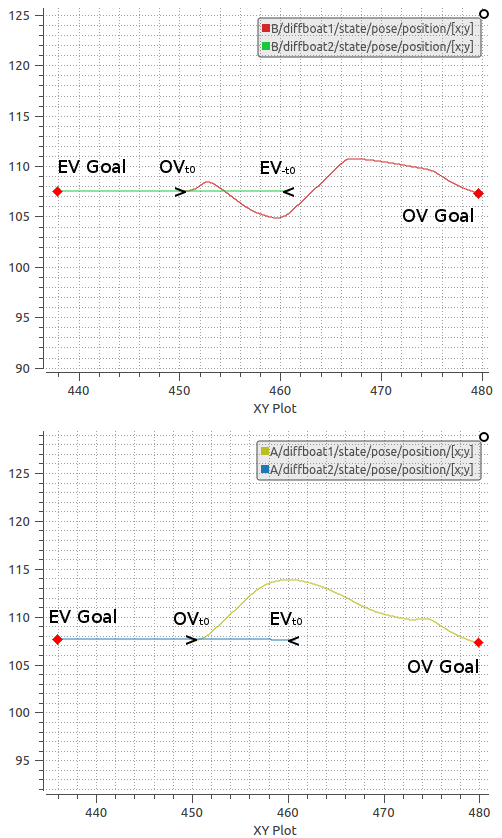
\includegraphics[scale=0.50]{figs/Result_HeadOn_With_Without_ATC.png}
        %     \caption{Head-on Scenario Simulation Result with \ac{ATC} vs without \ac{ATC}. Start positions are denoted by OV$_{t0}$ for own vessel and EV$_{t0}$ for encountering vessel. (A) Own vessel COLREGS-compliant behavior due to A* \ac{ATC} path planner. (B) Non COLREGS-compliant own vessel behavior generated by A* without \ac{ATC}.}
        %     \label{fig:Result_HeadOn_With_Without_ATC}
        % \end{figure}
        
        % \begin{figure}[H]
        %     \centering
        %     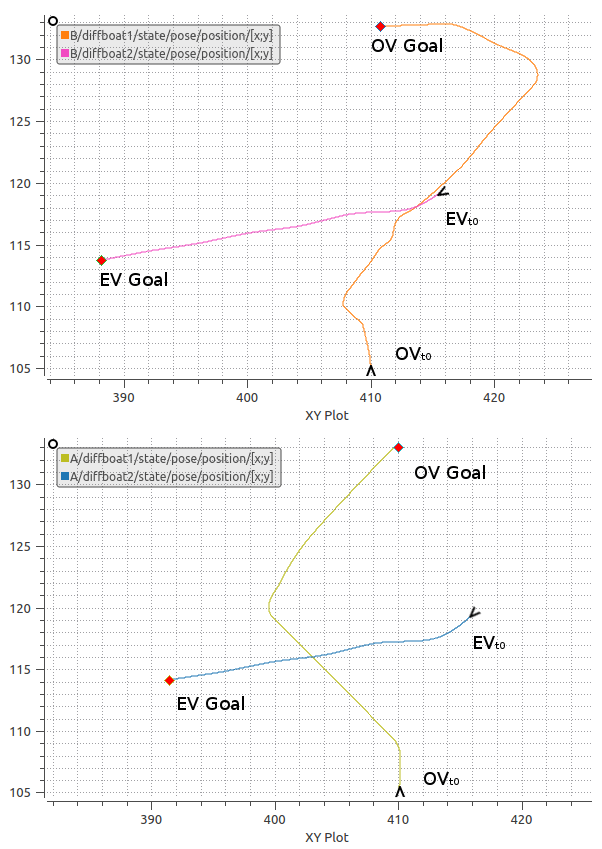
\includegraphics[scale=0.50]{figs/Result_CrossingRight_With_Without_ATC.png}
        %     \caption{Crossing from Right Scenario Simulation Result with \ac{ATC} vs without \ac{ATC}. Start positions are denoted by OV$_{t0}$ for own vessel and EV$_{t0}$ for encountering vessel. (A) Own vessel COLREGS-compliant behavior due to A* \ac{ATC} path planner. (B) Non COLREGS-compliant own vessel behavior generated by A* without \ac{ATC}.}
        %     \label{fig:Result_CrossingRight_With_Without_ATC}
        % \end{figure}
        
    % \begin{figure}[H]
    % \centering
    
    %     \begin{subfigure}[b]{0.5\textwidth}
    %       \centering
    %         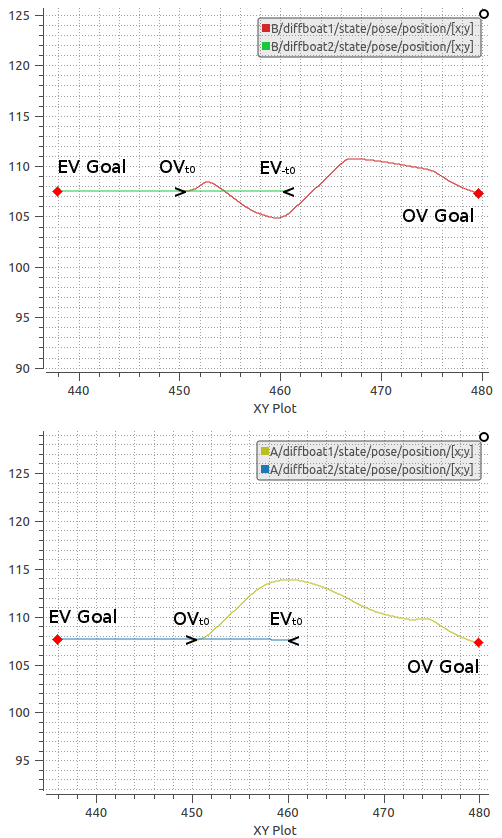
\includegraphics[scale=0.40]{figs/Result_HeadOn_With_Without_ATC.png}
    %         \caption{Head-on Scenario Simulation Result with \ac{ATC} vs without \ac{ATC}. Start positions are denoted by OV$_{t0}$ for own vessel and EV$_{t0}$ for encountering vessel. (A) Own vessel COLREGS-compliant behavior due to A* \ac{ATC} path planner. (B) Non COLREGS-compliant own vessel behavior generated by A* without \ac{ATC}.}
    %         \label{fig:Result_HeadOn_With_Without_ATC}
    %     \end{subfigure}
    %     \begin{subfigure}[b]{0.5\textwidth}
    %       \centering
    %         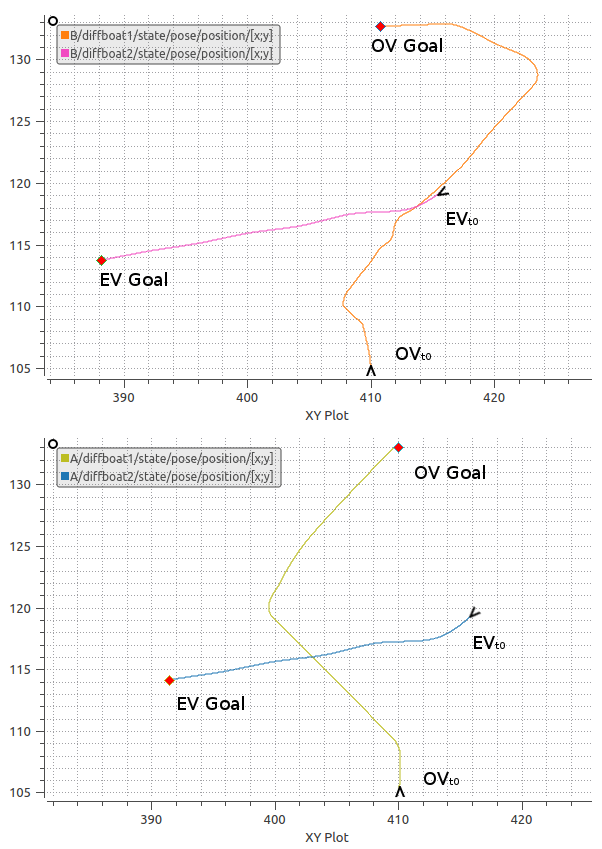
\includegraphics[scale=0.40]{figs/Result_CrossingRight_With_Without_ATC.png}
    %         \caption{Crossing from Right Scenario Simulation Result with \ac{ATC} vs without \ac{ATC}. Start positions are denoted by OV$_{t0}$ for own vessel and EV$_{t0}$ for encountering vessel. (A) Own vessel COLREGS-compliant behavior due to A* \ac{ATC} path planner. (B) Non COLREGS-compliant own vessel behavior generated by A* without \ac{ATC}.}
    %         \label{fig:Result_CrossingRight_With_Without_ATC}
    %     \end{subfigure}
    
    % \caption{Encounter scenarios for evaluation. Scenarios adopted from ~\cite{Huang2019Generalized}.}
    % \label{fig:simulation_uwsim_encounters}
    % \end{figure}
    
%AMA a diferenca entre avg e max eh enorme. explique bem o motivo disso. p um problema de tempo real, essa variacao nao eh muito interessante. 

\todo{cite authors on table caption}
\begin{table}
\caption{Based on \cite{} we made a quantitative evaluation of our planning system measuring computational cost and minimum distance between vessels.}
\centering
\begin{tabular}{|c|c|c|c|c|c|c|} 
\hline
\multirow{2}{*}{\textbf{Encounter} }                                                               & \multirow{2}{*}{\begin{tabular}[c]{@{}c@{}}\textbf{Scenario }\\\textbf{ Variation} \end{tabular}} & \multicolumn{3}{c|}{\begin{tabular}[c]{@{}c@{}}\textbf{Computational }\\\textbf{ Time (s)} \end{tabular}} & \multirow{2}{*}{\begin{tabular}[c]{@{}c@{}}\textbf{Successful }\\\textbf{ Avoidance} \end{tabular}} & \multirow{2}{*}{\begin{tabular}[c]{@{}c@{}}\textbf{Minimum }\\\textbf{ Distance (m)} \end{tabular}}  \\ 
\cline{3-5}
                                                                                                   &                                                                                                   & \textbf{Max.}  & \textbf{Average}  & \textbf{Std. Deviation}                                              &                                                                                                     &                                                                                                      \\ 
\hline
\multirow{3}{*}{\textbf{Head-On} }                                                                 & \textbf{No ATC}                                                                                   & 0.369          & 0.074             & 0.081                                                                & Yes                                                                                                 & 4.431                                                                                                \\ 
\cline{2-7}
                                                                                                   & \textbf{ATC}                                                                                      & 0.364          & 0.076             & 0.076                                                                & Yes                                                                                                 & 1.599                                                                                                \\ 
\cline{2-7}
                                                                                                   & \textbf{Wind}                                                                                     & 0.355          & 0.077             & 0.079                                                                & Yes                                                                                                 & 1.505                                                                                                \\ 
\hline
\multirow{3}{*}{\begin{tabular}[c]{@{}c@{}}\textbf{Crossing }\\\textbf{ from Right} \end{tabular}} & \textbf{No ATC}                                                                                   & 0.390          & 0.050             & 0.098                                                                & Yes                                                                                                 & 5.414                                                                                               \\ 
\cline{2-7}
                                                                                                   & \textbf{ATC}                                                                                      & 0.395          & 0.052             & 0.104                                                                & Yes                                                                                                 & 3.264                                                                                                \\ 
\cline{2-7}
                                                                                                   & \textbf{Wind}                                                                                     & 0.403          & 0.085             & 0.124                                                                & Yes                                                                                                 & 3.739                                                                                                \\ 
\hline
\multirow{3}{*}{\begin{tabular}[c]{@{}c@{}}\textbf{Crossing }\\\textbf{ from Left} \end{tabular}}  & \textbf{No ATC}                                                                                   &           &              &                                                                &                                                                                                &                                                                                                 \\ 
\cline{2-7}
                                                                                                   & \textbf{ATC}                                                                                      &               &                   &                                                                      &                                                                                                     &                                                                                                      \\ 
\cline{2-7}
                                                                                                   & \textbf{Wind}                                                                                     &                &                   &                                                                      &                                                                                                     &                                                                                                      \\ 
\hline
\multirow{3}{*}{\textbf{Overtaking} }                                                              & \textbf{No ATC}                                                                                   &   0.368             &  0.006                 &  0.030                                                                    &   Yes                                                                                                  &  3.325                                                                                                    \\ 
\cline{2-7}
                                                                                                   & \textbf{ATC}                                                                                      & 0.357          & 0.018             & 0.022                                                                & Yes                                                                                                 & 3.101                                                                                                \\ 
\cline{2-7}
                                                                                                   & \textbf{Wind}                                                                                     & 0.852          & 0.039             & 0.073                                                                & Yes                                                                                                 & 1.787                                                                                                \\
\hline
\end{tabular}
\label{tab:results}
\end{table}

    % Grammarlly: 100/100
    Agrawal \etal ~\cite{Agrawal2015COLREGS} evaluate theirs A* approach in a 100mx100m grid with a resolution of 1:1, resulting in a search space of 10000 cells, we built our scenarios respecting the same proportionality. In all scenarios, our \ac{USV} plan in a 20mx20m grid with 1:0.2 resolution, resulting in a search space of 10000 cells. The choice of 20x20 dimension is related to real limitations of the range and reliability on laser sensors, the RPLIDAR A3 laser~\cite{RPLidarA3} model, for example, is reliably capable of detection in a 25 meters distance range.